\documentclass[fr]{../../../eplsummary}

\usepackage{gensymb}

\hypertitle{Offshore Geotechnics}{8}{GCIV}{2074}
{Thomas Wyckmans}
{Benoît Spinewine}

\newpage

\part{Introduction}

Utile dans différents domaines :
\begin{itemize}
    \item Shipping
    \item Renewables energy
    \item Oil \& Gas
    \item Water supply / Desalineation
    \item Deep-sea mining
    \item ...
\end{itemize} 

La jonction continent-eau, consiste en une bordure ("shelf") jusqu'à 100m de profondeur, suivi d'une pente et finalement un redressement jusqu'à arriver dans les plaines abyssales des eaux profondes.

\begin{center}
    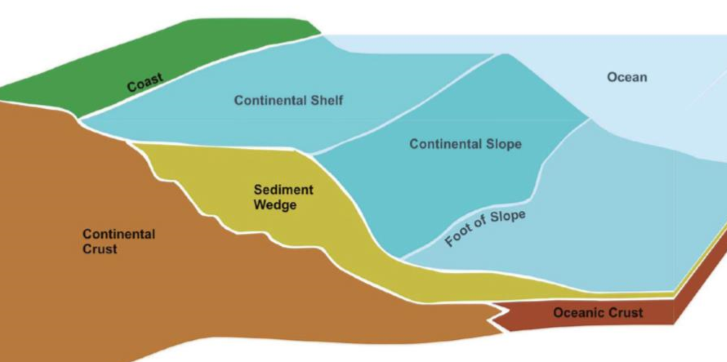
\includegraphics[scale=1]{pictures/introduction/photo1.PNG}
\end{center}

Si il n'y avait pas de bordure, les sédiments apporté par les cours d'eau sont dispersé par les courants marins pour en former une.

On construit généralement sur la bordure continentale, il arrive de construire sur la pente, mais il y a de gros risques de glissements.

Il existe des lieux sans bordure (Taiwan's eastern coast, ...).

Il existe deux type de jonction entre les continents :
\begin{itemize}
    \item Active Margin
    \item Passive Margin
\end{itemize} 

\begin{center}
    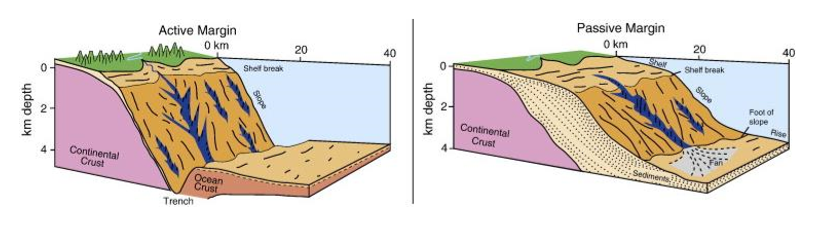
\includegraphics[width=\linewidth]{pictures/introduction/photo2.PNG}
\end{center} 

\underline{Définition :} une structure offshore n'a aucun accès à la terre et peut être soit fixée au sol soit flotter. Elle est définie par deux paramètres importants : 
\begin{itemize}
    \item fonction : forage, production, stockage, transport
    \item configuration : fixé, flottante
\end{itemize} 

\section{Fonction}

\subsection{Production}

Ce type de plate-forme reste localisée au même emplacement durant toute leur "vie" (\~ 20 30 ans). Dans les eaux peu profondes elles sont fixées (jacket platform) alors que pour les eaux profondes (>1000 ft) il devient économiquement intéressant de les faire flotter. 

\subsection{Storage}

Pour les structures offshore éloignée des côtes, les pipelines n'ont plus d'intérêt économique. On stocke parfois les ressources sur des plate-forme utilisant une base en béton (gravité) pour ensuite les transporter par bateau. On utilise également souvent des "ship-shaped floating" pour décharger une structure.

\subsection{Transportation}

on peut utiliser des pipelines ou des bateau tank pour les localisations plus éloignées.

\section{configuration, fixed}

\begin{figure}[!ht]
    \centering
    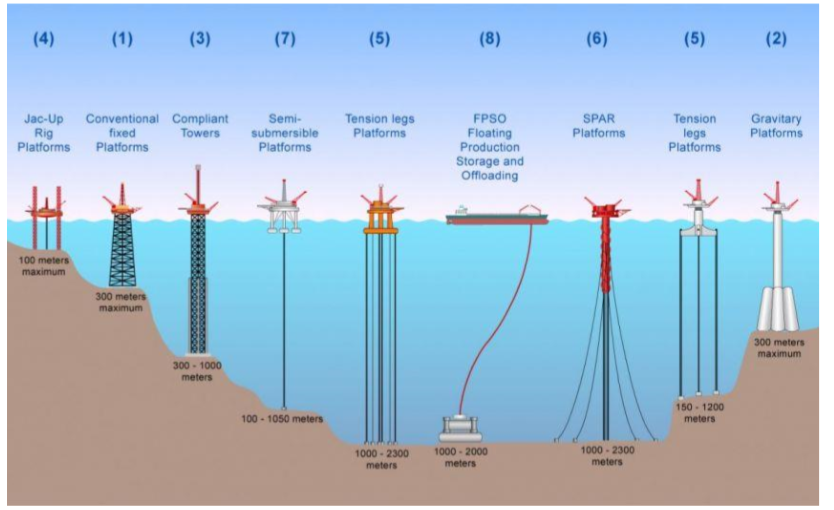
\includegraphics[width=\linewidth]{pictures/introduction/photo3.PNG}
\end{figure} 

\subsection{Jacket Structure}

Ce sont les structures les plus courantes pour le forage et la production. Elles sont construites "onshore" puis déplacée dans l'eau, elles peuvent tenir 20-30 ans. Elles sont dimensionnées sur base de la profondeur et des forces dynamiques (vagues, vent, courant, ...). Elles ont entre 3 et 8 jambes battues dans le sol pour éviter le renversement. Elles sont intéressantes jusqu'à 1700 ft (\~ 100m).

\subsection{Compliant tower}

Similaire au "Jacket Platforms" mais plus économe (utilise moins d'acier pour une même profondeur), consiste en une tours flexible et un pont d'opération pour forer/produire. Elles sont dimensionnées pour supporter de grosse déviation \& forces latéral. 

Elles sont épinglées ("pinned") aux fonds marin avec des pieux de manière à permettre une certaine flexion. Certaines sont haubané pour éviter de trop gros balancement.

\subsection{Gravity Base Structure}

Très pratique pour la production ou le stockage. Elles sont généralement placée à proximité de la rive et tenu en place par leur poids propre, on a donc pas besoin d'ancrage ou de pieu. Il faut une grande masse volumique, on utilise du béton. 

\subsection{Jack-up barge}

Plate-forme pouvant être élevée au dessus du niveau de l'eau. Utilisé pour des forages à cours terme, concue pour aller de site en site. Composé de trois jambes en acier (3D portal frame). Pendant le forage, elle est stationnaire. On peut les utiliser pour des profondeurs de \~ 400 ft. 

\subsection{Satellite platform}

Petite plate-forme utilisée en eau peu profonde, elles servent d'annexes (héliport, centre de secours, ...). Elles sont supportées par des trépieds foré à leur base. 

\section{Configuration, floating}

\subsection{Drillship}

Il s'agit d'un bateau qui a été affreté avec un mât de charge (derrick) et différents appareils de forage. Surtout utilisé pour trouver de nouveau lieu de forage. Ils utilisent des système de maintient dynamique pour rester stable sans avoir recours à un ancrage.

\subsection{Semi-submersible}

Il y a une partie qui est immergée et qui sert de flotteur à la structure. Elles peuvent être déplacée facilement. Elles peuvent utiliser un système de maintient dynamique mais sont généralement ancrée pendant les opérations de forage. Utilisable entre 600 et 6000 ft.

\subsection{FPSO, FSO}

FPSO : Floating, Production, Storage and Offloading. Elles sont surtout utilisée en dernier recours (pipeline et structure fixée ne sont pas économique). Elles ne sont pas designée pour le forage.

\subsection{SPAR}

Dimensionné pour supporter un forage ou une opération de production en eau profonde. elles sont ancrée au fond marin avec des "mooring" lines. Il en existe deux type: classic \& truss Spars. Ces plate-forme on la possibilitée de se déplacer horizontalement.

\subsection{TLP (Tension Leg Platform)}

Plate-forme avec une flottaison verticale surdimensionnée qui est contrée par des amarres. Utile jusqu'à 6000ft. Il en existe des version réduites relativement peu cher utilisable entre 600 et 3500 ft (elles sont également utilisable comme satellite ou de plate-forme de préproduction pour des découverte en eau profonde). Le SPAR reste plus économique pour la construction de petites et moyennes plates-formes, a une meilleur stabilité (grâce à son contrepoids) et ne dépend pas d'un "monitoring" pour rester stable.

\section{Configuration, Subsea Structures}

\subsection{Wellhead}

il s'agit de la fin d'un tube de forage, il comprend un moyen de suspendre les tubes de production et d'installer "l'arbre de noel" en préparation du forage.

\subsection{Christmas Tree}

Comprend un ensemble de valves et de jauges qui contrôle le flux de combustible dans le forage. Il peut être considéré comme sec ou mouillé en fonction de sa localisation (onshore/offshore).

\subsection{Manifold}

Permet de diriger un flux sortant de plusieurs têtes de forage en différentes lignes de productions. Il a parfois recours à des "skirted fondation" ou à des pieux pour être supporté par les fonds marins.

\subsection{Sleds, PLETs and PLEMs}

Différentes partie du système qui lie les différents lignes de production ensemble.

\subsection{SURF (Subsea Umbilicals, Risers and Flowlines)}

Généralement utilisée pour désigner les pipelines et autres équipement connectant le système sous marin au système flottant. On utilise pour ça des tubes flexible et énormément de capteurs, câbles, ... pour surveillé la pression, la température, ... 

\section{Type of fondation}

\subsection{Gravity based foundations}

Avec ou sans jupe, nécessaire pour certain site (fjords, lochs, ...). Adapté à des sols à grande résistance (argile surconsolidé ou des sables).

\subsection{Spudcan}

Utilisé pour les "jack-up plate-forme", d'un diamètre d'environ 15m. Dans un sol dur, on aura une pénétration partiale, dans un sol mou on aura une grande pénétration (\~ 30m). Il y a un risque de "punch-through".

\subsection{Autre}

\begin{itemize}
    \item Mudmats
    \item Sliding mudmats
    \item Skirted foundations
    \item Applicable to mudmats, GBFs, spudcans
    \item Suction anchors/caissons
    \item Anchor foundations (VLAs, SEPLAs, ...)
    \item torpedo anchors
    \item ...
\end{itemize}

\newpage 

\part{Site investigations}

\section{Marine sediments}

\subsection{origine}
    
    \begin{itemize}
        \item Terrigène (terrigenous): qui date d'il y a très longtemps
        \item Litaugène (litaugenous): résultats de l'érosion
        \item Biogène (Biogenous): silica dissout ou composition de calcaire (shells, skelettons)
        \item Hydrogène (hydrogenous): précipitation de minéraux dissout.
        \item Pelagic (je crois) poussère due au courrants marin.
    \end{itemize} 
    
\subsection{Mineralogie}
    
    On trouve en majorité du sable silicieux (robust, non cassable), des carbonates silicieux (faible, cassable) et des argiles marines.
    
    \begin{center}
    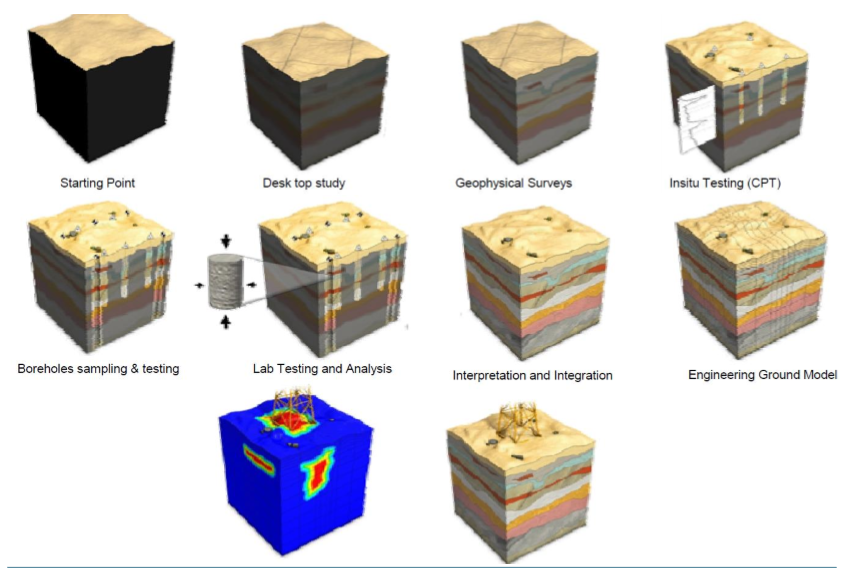
\includegraphics[width=\linewidth]{pictures/part2/photo1.PNG}
\end{center} 

\section{Desktop Study}

Etude des données existantes pour une évaluation préliminaire du site. Elle inclut : bathymetry, géologie de la région, geohazards potentiels, obstacles possibles et les données océanographiques de la région.

De plus, l'étude en bureau permet de formuler explicitement ce qu'on a besoin en terme d'étude géotechnique et géophysique en déterminant les données manquantes. Cela permet de cibler les points d'intérêts.

L'étude inclus une gestion des risques (geohazards (sismic, submarines slides,...)

Les données océanographiques de la région permette une meilleur compréhension des courants, des vents, ... et d'ainsi plannifier au mieux les dates d'investigations futurs et le lieu d'installation de la plate-forme. D'autres informations seront récupérée par la suite, mais c'est une bonne base de travail.

Cette étape peut durer plusieurs mois en fonction de la taille du projet mais est nettement moins cher que les étapes suivantes.

Attention au zonage, toujours regarder autours pour être certain qu'on est pas dans une "anomalie".

\section{Geophysical investigation}

Le but de cette partie est de rapidement décrire les différents équipement disponible et leur capacités. Ils se concentrent sur trois objectifs : 
\begin{itemize}
    \item la profondeur, la hauteur d'eau
    \item les élément du fond marin
    \item les sédiments de la stratigraphie
\end{itemize} 

Donne des indications local sur le seabed et de large indication sur le type de sol. On obtient les grandes lignes de la stratification et les différents obstacles. La fréquence du signal va faire varier la résolution. On peu même révéler la présence de poche de gaz peu profonde ou d'hydrate de méthane.

Une investigation type inclue au minimum :
\begin{itemize}
    \item Bathymetry
    \item Seismic reflection (stratigraphie des fonds marins)
    \item Side-scan sonar (seabed topographie, "pock marks \& ice gouges")
\end{itemize} 

Les données géophysique demande généralement une vérification pour être utilisable en géotechnique de manière quantitative. Elles restent néanmoins primordiale à la création d'un modèle de seabed.

Ce type d'investigation peu durer 3 mois et coûter environ un million de dollar (US).

\subsection{Bathymetric mapping}

Utilisé pour quantifier la profondeur et fournir un image 3D du seabed. Fourni des information intéressante sur la surface du terrain (pente, crevasse, débris, volcans, ...).
Il en existe deux type : "echo sounding" \& "swathe bathymetry". 

\subsubsection{Echo sounding}

Similaire à un "echo sounders" classique, seulement celui-ci doit en permanence corriger les erreurs du a l'état de la mer, l'équipement doit être correctement calibré en fonction de la vitesse de l'eau.

Il est possible d'obtenir une bathymétrie plus précise en utilisant un "multi-beam echo sounding". C'est plus efficace en terme de temps et de coût. Généralement utilisé sur des ROV (remotely operated vehicle), on utilise alors un positionnement GPS pour connaitre la position précise de l'instrument.

\subsubsection{Swathe bathymetry}

Le bateau balaye le fond marin avec un scanner (gauche à droite ou d'avant en arrière) et récolte ponctuellement un grand nombre d'informations. Il faut ensuite un logiciel pour transformer ces donnée en image 3D. C'est très utile dans des terrains accidenté. Peut être également utilisé depuis un ROV. En moyenne, cela couvre 4 fois la profondeur.

\subsection{Sea floor mapping}

La sonde génère une impulsion d'énergie à la fois et attend que le son soit réfléchi. La plage d'imagerie est déterminée par la durée d'attente du remorqueur avant de transmettre la prochaine impulsion d'énergie acoustique. L'image est ainsi construite en une ligne de données à la fois. Les objets durs réfléchissent plus d'énergie, provoquant un signal sombre sur l'image, les objets mous qui ne reflètent pas l'énergie apparaissent aussi comme des signaux plus légers. L'absence de signal sonore montre une zone blanche.     

\subsection{Subseabed continuous seismic profiling}

\begin{center}
    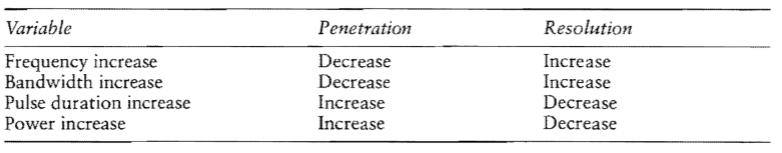
\includegraphics[width=\linewidth]{pictures/part2/photo3.PNG}
\end{center} 

Un système de profilage est composé de trois composantes: une source sonore, une matrice de récepteurs et un enregistreur. La source et les récepteurs sont généralement remorqué à quelques mètres sous la surface de l'eau. L'objectif ultime est un outil qui offre une pénétration maximale avec une haute résolution (capable de définir des couches minces). Ces deux objectifs sont mutuellement exclusif et par conséquent il faut trouver un compromis. La matériel moderne ce rapproche de cette idéal mais est très cher et n'est donc pas toujours justifié  pour une simple étude d'emplacement.

Le degré de pénétration est finalement contrôlé par la composition du fond de la mer et des couches sous-jacentes. De fortes couches près de la surface empêche la pénétration des ondes. On détermine le type de sol par la quantité d'énergie dispersée par les fonds marins.

De plus, le type d'outil doit être sélectionné en fonction de l'application spécifique, les différentes sources sismiques sont désignées par des noms qui reflètent leur puissance et leur fréquence.

\begin{center}
    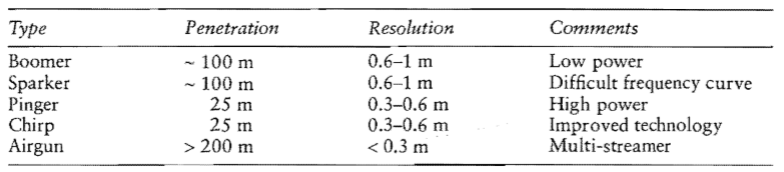
\includegraphics[width=\linewidth]{pictures/part2/photo4.PNG}
\end{center} 

Une autre méthode consiste à créer un signal acoustique plus propre (utilisation de pistolet à air).

Finalement, on peut faire varier la profondeur de la sonde tractée, il sera ainsi plus facile de gérer les réflexions de la surface de l'eau. Ce système sera plus affecté par les états marin pauvre.

\subsection{Autonomous underwater vehicles}

On utilise des AUV (véhicules sous-marins autonomes), il ne faut plus utiliser de câble ombilical pour transmettre les informations (ROV). Elles sont stockée et récupérée en même temps que le véhicule ou par modem accoustique (à travers l'eau). 

Il en existe différents modèles :

\begin{itemize}
    \item Side Scan Sonars : fournit une image du seabed sur base de la distribution des sédiments, la détection d'object et leur hauteur si base de trigonométrie. Pratique mais doit être proche du seabed, est très sensible à la météo et à son positionnement.
    \item Sub-bottom Profilers
    \item UHR shallow seismic refraction with stop and go seabed system (GAMBAS)
\end{itemize}

\subsection{Survey line layout}

Ce plan est conçu pour capturer les zones d'intérêts :
\begin{itemize}
    \item installations sous marines
    \item les mouillages et les bouées
    \item emplacements possibles des plate-formes
\end{itemize}

On fait des enquêtes annexes pour les pipelines.

Un navire fait ce plan en naviguant sur la grille définie en recueillant les données nécessaires.

Lorsqu'une étude de forage existe déjà, il est important d'établir un lien pour permettre au géophysiciens de calibrer les données d'arpentage par rapport aux données de forage. Cela permet de directement réexécuter une lignes si nécessaire sans dépenses significatives. Le maillage peu être adapté en fonction des zones présentant un intérêt particulier.

\subsection{Example of seabed and sediment profiling and hazard assessment}

Les grands objects tels que les rochers, les pinacles, les crêtes et les ondes de sable sont de bons réflecteurs et produisent une zone d'ombre acoustique derrière laquelle aucune réflexion n'est générée.

La force de rétro diffusion du matériau peut également fournir une indication du type de matériau (élevée = calcarénite ou gravier, faible = sables boueux). Cette interprétation peut être moins subjective si accompagnée d'échantillons ou de carottes de fond.

L'une des applications les plus importantes est de localiser les récifs coralliens ou les pinacles coralliens.

les formes de lit telles que les ondulations du sable sont des manifestations des courants dominants. De petites marques de fourmillement peuvent également être observées et sont souvent une indication d'un effondrement dû à l'échappement de gaz.

\subsubsection{Local hazard assessment}

Les plates-formes auto-élévatrices placées le long des installations existantes aux fins de travaux nécessitent des informations sur la pénétration des spudcans.

Les installations sous-marines sont relativement petites dans la zone du plan et sont généralement sensibles aux irrégularités du fond marin.

Même les cicatrices causées par l'ancrage des ancres de dragage peuvent poser des problèmes, étant donné le volume important de sol perturbé.

Les irrégularités locales du fond marin peuvent également entraîner un tassement différentiel excessif pendant la durée de vie de la structure et, dans le cas des structures de base en béton, les composants structuraux de la base peuvent être surchargés ou nécessiter un coulis de fondation.

\subsubsection{Regional hazard assessment}

Les zones de changement significatif de la profondeur de l'eau, avec des gradients élevés, sont particulièrement vulnérables aux forces naturelles telles que les tremblements de terre et les courants océaniques élevés qui peuvent provoquer une instabilité des pentes ou des coulées de boue. 

On analyse des échantillons et on date les sédiments pour établir la fréquence des ruptures de pente et la dispersion des débris par les courants océaniques.

\section{Geotechnical investigation}

Ce type de recherche combine un travail offshore et des tests d'échantillons en laboratoire. Certains tests sont fait directement sur place (penetration, vane shear testing).

Cette étape à pour but de valider la théorie avancée par les deux étapes précédentes donnant des données beaucoup plus précises sur la stratigraphie (ponctuellement). Si celle-ci sont juste, on peut intégrer les résultats obtenu pour les différents à des zones beaucoup plus grande, on considérant bien entendu une diminution de précision en fonction de la distance.

\begin{center}
    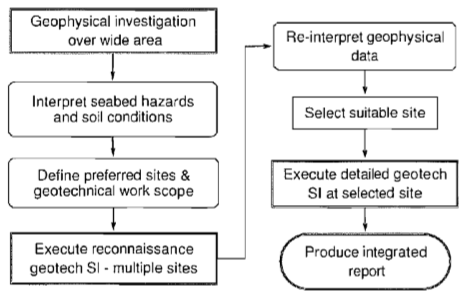
\includegraphics[scale=1]{pictures/part2/photo2.PNG}
\end{center} 

Ce type d'investigation peut durer au minimum 3 mois (dépend de la taille du bateau et sa capacité de forage) mais dépasse souvent 1 an. Le budget peut revenir à plusieurs million de dollars (US) car cela dur longtemps et les bateaux sont chers.

\subsection{Choice of investigation system}

Parfois seul une étude géotechnique est effectuée afin de réduire les coûts ou en raison de la petite étendue du site à étudier.

Une étude de site géotechnique est réalisé par un équipement spécialisé à partir d'une plate-forme construite à cet effet. Il existe deux système alternatifs: fond de trou (downhole) \& fond marin (seabed). Il exist plusieurs type de forage en fonction de l'endroit de départ du travail a effectuer (bateau ou plate-forme).

Fond de trou est typiquement utilisé dans l'industrie pétrochimique. Cependant en géotechnique, les forages doivent être effectuées de manière beaucoup plus sensible. En revanche, un système de fond marins comprend des équipement qui reposent sur le fond marin. La profondeur maximale d'investigation est inférieur à celle d'un fond de trou. Mais la flexibilité et le contrôle accru des systèmes des fonds marins offrent de nombreux avantages.

L'équipement doit être capable de résister aux pressions hydrostatiques élevées et doit être adapté aux type de sédiments, un outil se comporte différemment dans l'argile molle que dans le sable dense.

\subsection{Investigation platforms}

Le choix de la plate-forme appropriée dépend de la profondeur de l'eau. Cependant, de plus petites options influenceront la capacité à entreprendre une portée de travail appropriée. Les différents possibilités sont :

\begin{itemize}
    \item Support vessel or barge (<20m)
    \item Jack-up rig (20-120m)
    \item Support vessel (depends on the vessel draft)
    \item Specialised drilling vessel (>20m)
\end{itemize}

Généralement, les capacités d'ancrage des navires sont limitées à des profondeurs <200m, les navires positionnés dynamiquement sont plus appropriés pour les eaux profondes. Ces navires sont très cher, ils ne sont donc utilisé que dans les zones ou ils peuvent être stationné de façons quasi permanente. 

\subsubsection{Low draft barges}

Capable de travailler dans les eaux peu profondes. Adaptés aux enquêtes sur les pipeline. Un système d'amarrage multipoints (min 3 ancrages) est nécessaire pour garder le bateau en place. Il faut faire attention au fort courant dans les tronçons peu profond entre les îles.

\subsubsection{Support vessels}

Capable de déployer des équipements télécommandés. On a également recours à un amarrage multipoints. Seuls des équipements à faible faible risque peuvent être déployé. Les dommages matériels seraient excessivement coûteux si le navire quittait soudainement son emplacement. En sachant qu'il coûte déjà des dizaines de milliers de dollars US par jour. 

\subsubsection{Dynamically positioned vessels}

Adapté aux travaux en eaux profonde, aux études qui nécessitent l'étude de grandes zones et aux études de pipelines. Bon maintient de position (redondance), moins de danger d'endommager l'équipement. Souvent muni d'une moon pool pour pouvoir utiliser un équipement de forage en parallèle d'un équipement télécommandé. Il faudra néanmoins s'assurer un équipement de compensation de soulèvement lors de forage. Ce n'est pas prévu de base. On peut également ajouter un dispositif de forage qui peu être utilisé sur le côté ou la poupe du navire. Le tarif journalier est dans les dizaines de milliers de dollars US par jour mais reste le moins coûteux en eau profondes. 

\subsubsection{Specialised drilling vessels}

Auto-ancrage ou DP, ils sont auto-suffisants. Permet un travail de haute qualité pour les travaux géotechniques et en particuliers l'études des eaux profondes. Possède une moon pool et d'un système de compensation de soulèvement à liaison rigide (lié au fond marin). Pas d'apport d'eau clair, cela limite les fluide utilisable car ils doivent être utilisable avec de l'eau de mer. Coûts très élevée, il est donc intéressant d'en profiter pour faire différentes enquêtes en même temps.

\subsubsection{Jack-up rigs}

Offrent une plate-forme stable mais soumise à certaines limitations :
\begin{itemize}
    \item Par rentable de forer plus d'un trou car demande beaucoup d'effort à déplacer
    \item Il n'est généralement pas possible d'effectuer une enquête en même temps que l'installation d'activité pétrolière régulière, contrainte d'espace.
    \item Profondeur limite de 120m (augmente avec la taille des plate-formes).
    \item tarifs élevé (centaine de milliers de dollars US) et soutient logistique important (hélicoptère, ...).
\end{itemize}

C'est donc rarement choisit, sauf dans les installations proches des côtes.

\subsubsection{Semi-submersible drilling rig}

Efficace en eau profonde mais très cher. (>250 000 \$). Navire encré en fond de mer, ce qui augmente encore le coût en terme de temps. Il est possible de déplacer le navire sur l'ancre, sans déplacer les ancrages et donc forer plusieurs trous. Ce type de plate-forme est rarement utilisée pour les investigations géotechniques.

\subsection{Drilling and coring system}

\subsubsection{Manual and remote subsea systems}

Dans des eaux peu profondes, les opérations de forage et d'échantillonnage peuvent être effectuées par des plongeurs. Le problème est que les plongeurs ne sont pas toujours des ouvriers qualifiés, il faut donc monitorer la qualité du forage.

Depuis 2005 on utilise un système d'investigation géotechnique sous marin robotique (PROD). Il peu prélever des carottes de roche ou des échantillons de sol et effectuer des essais pénétromètres in situ jusqu'à 100m de profondeur (et 2000m dans les eaux profondes). 

\subsubsection{Jack-up rigs}

Elle dispose généralement de matériel de forage, mais il reste moins cher de prendre des outils onshore et de les positionner sur la plate-forme. Cela permet d'obtenir des carottes de grande qualité. On peut également y placer un pénétromètre à cône. Il ne faut pas oublier qu'il est très onéreux de déplacer la plate-forme pour faire un deuxième test. La taille de ces plate-formes permet énormément de stockage, large choix de fluide de forage.

\subsubsection{Specialised drilling vessels and semi-submersibles}

La majorité des tests sont effectués avec cette solution. Il faut pouvoir compenser les déplacement, avoir un trépan ouvert sur l'ensemble du trou inférieur (ne veut rien dire = "Open drag bit on bottom hole assembly "), utilisation d'outils ombilicaux ou filaires et finalement "Seabed guide base with clamp" (pas compris non plus).

Ces éléments sont relativement standard sur des bateaux géotechniques.

On va rapidement décrire les différents éléments trouvable sur les bateaux :

\underline{Seabed guidebase and heave compensation :} voir p85. 

\underline{Drilling bit and pipe :} Le poids nécessaire est fourni par des bagues de forage. Contrairement à une installation de forage d'exploration, il est nécessaire de pouvoir régler les compensateurs de mouvement de façon à ce qu'ils réagissent de manière suffisamment sensible pour le type de sol et minimisent ainsi la perturbation du sol en dessous.

\underline{Umbilical cable :}  permet de visualiser les données en temps réel et ainsi d'avoir un contrôle direct sur le test.

\underline{Downhole tool :} p86 

\underline{Rock coring :} permet de récupérer des roches et sinon bah c'est du baratin

\underline{Wheel drive :} à la base permet de faire un essai CPT depuis les fonds marins grâce à sa masse relativement importante. Le cadre peut être modifié pour accueillir des éléments de carottage rocheux. Utile pour les eaux profondes ou l'on s'intéresse principalement au 20-50 premiers mètres.

\subsection{In situ testing equipement}

\subsubsection{Cone penetrometer}

Le test de pénétration au cône (CPT) est actuellement l'essai in situ le plus réalisé lors d'une étude géotechnique, utilisant généralement un piézocône qui intègre la mesure de la pression interstitielle. Cela mesure la résistance à la pénétration, qui est généralement exprimée comme la force par unité de surface qc. Un manchon est monté au-dessus de la pointe et une cellule de charge attachée à ce mesure le frottement latéral, à nouveau exprimé en force par unité de surface fs. Les piézocônes ont également un transducteur de pression qui mesure la pression de l'eau. Le taux de pénétration standard est de 20 mm / s, soit environ un demi-diamètre par seconde, bien que l'équipement moderne soit généralement capable de faire varier le taux d'au moins un ordre de grandeur.

 La capacité du cône est généralement de 10 ou 15 tonnes, bien que la poussée maximale puisse être limitée par le poids de la structure du fond marin.  Le piézocône est principalement un outil de profilage et les résultats peuvent être utilisés pour déterminer les types de sol des différentes couches interceptées. Puisque les données sont obtenues en continu avec la profondeur, il est capable de détecter de fines modifications de la stratigraphie.
 
 \underline{Corrections to measured cone resistance :}
 
 $$ q_t = q_c + (1+\alpha)u_2 $$ 
 
 $\alpha$ est le "area ratio". Il peut être calculé sur base des dimensions physiques du cône. Il est généralement défini en laboratoire.
 
 Un autre ajustement est nécessaire, pour distingues la composante de surpression de la résistance "net" du cône ($q_{net}$).
 
 $$q_{net} = q_t - \sigma_{v0} = q_c + (1-\alpha)u_2 - \sigma_{v0} = q_c - \sigma_{v0}'-\alpha u_0 + (1-\alpha)\Delta u_2$$ 
 
 avec $\sigma_{v0}$ la surcharge totale et $\Delta u_2$ la différence de pore water pressure. Généralement négligeable dans les sols avec une assez grande perméabilité, mais indispensable dans les argiles mou.
 
 Notez que ces corrections sont effectuées en prenant les conditions dans lesquelles les lectures du cônes on été prises. En effet, il faut discerner un fond marin d'un fond de trou.
 
 \underline{Soil type characterisation :}
 
 on étudie : 
 \begin{itemize}
     \item Résistance à la pointe normalisée : $Q = q_{net}/\sigma'_{v0}$
     \item Ratio d'excès de pression interstitielle : $B_q = \Delta u_2/q_{net}$
     \item Ratio de frottement : $F_r = f_s / q_{net} $
 \end{itemize}
 
 Le principe général est que les sols les plus fort (sable dense ou "cemented sediments") on aura un grand Q et un petit $F_r$ comparé aux argiles.
 
 En général, les argile doux ou moyens (force) donneront un pression interstitielle élevée, un $B_q$ proche de 0.3-0.7 et un $F_r$ de 2 à 5\%.
 
 Quelques normes pour $F_r$ : 
 \begin{center} Clay > 4\%, Silt 2-3\%, Sand < 1\%, Peat (tourbe) > 8\%  \end{center}
 
 Abaque de Robertson : 
 
 \begin{center}
    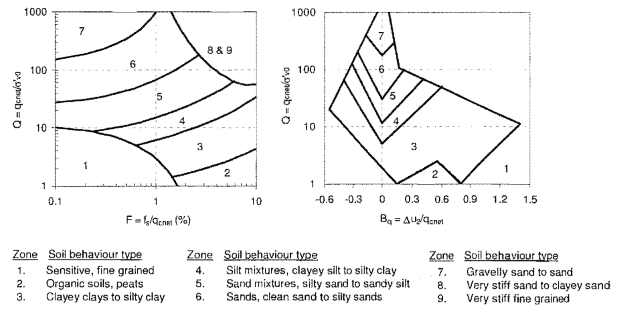
\includegraphics[scale=1]{pictures/part2/photo5.PNG}
\end{center} 

En considérant la pression interstitielle :

\begin{center}
    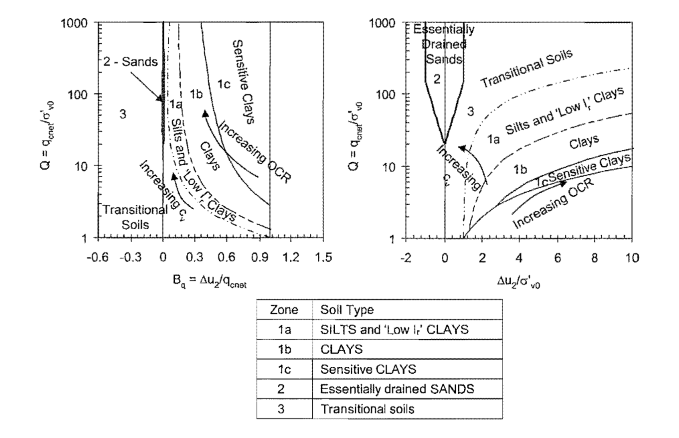
\includegraphics[scale=1]{pictures/part2/photo6.PNG}
\end{center} 

 \subsection{Sampling equipment}
 
 \subsubsection{Grab samples and box cores}
 
 Surtout utilisé pour la mise en place de pipelines où les 50 premier cm de sol sont critique. L'échantillon est remanié, on ne peu que avoir une analyse minéralogique. Utile pour le "model testing": mini-penetrometer,...
 
 \subsubsection{Drop cores and vibro-cores}
 
 On fait tomber un tuyau qui s'enfonce par gravité (6-8m de long et 100 mm de diamètre externe pour 85 mm interne). En haut du tube se trouve une masse de 500 à 1000kg. On laisse tomber l'engin de 10m au dessus du niveau d'eau. Dans les sols plus compacte, on remplace la masse par un vibreur électrique (et on met un diamètre plus grand). L'échantillon est relativement remanié. 
 
 \subsubsection{Seabed piston cores}
 
 Permet d'améliorer la qualité de l'échantillon. La succion développée entre le tube et le sol aide celui-ci à s'enfoncer. On incorpore ce type de piston aux carottier à gravité. Il y a un peu de remaniement, mais ils sont limité aux côtés de l'échantillon. Pour les sédiments mou, le carottier pénètre par son simple poids suffisamment profondément, il n'y a donc pas d'intérêt financier ni temporel à utiliser un piston.
 
 \subsubsection{Borehole samples}
 
 On fore comme en onshore.
 
 \newpage
 
 \part{Soil response \& Shallow foundations}
 
 \section{CPT acquisition}
 
 \underline{Alpha factor :} c'est la relation entre l'air du cône ou la pression de l'eau n'agît pas, et l'air du cône ou la pression agît. Cela reflète l'influence de la pression d'eau sur le cône.
 
 $$ \alpha = \frac{A2}{A1} $$ 
 
 \begin{center}
    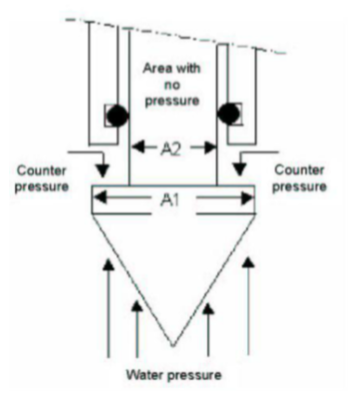
\includegraphics[scale=1]{pictures/part3/photo1.PNG}
\end{center} 

\underline{Beta factor :} c'est le facteur de correction de la pression d'eau juste devant et juste derrière la pointe du cône. Il peu se calculer ainsi :

$$ \beta = \frac{u_2 + u_{ol} - u_o}{u_1 + u_{ol} - u_o} $$ 

avec $u_o$ : la pression hydrostatique sur le cône relatif au fond marin et $u_{ol}$ : la pression hydrostatique au fond du puits de forage.

\section{Bearing capacity for shallow foundation}

\subsection{Rappels}

\subsubsection{Mohr - Coulomb}

Exprime une résistance au cisaillement $\tau_c = c + \sigma' tan \phi$ qui augmente linéairement avec la contrainte normale effective $\sigma' = \sigma - u$. 

\subsubsection{Sol en rupture par butée et poussée}

... 

\subsubsection{Capacité portante d'une fondation superficielle}

\underline{Hypothèses :}
\begin{itemize}
    \item Sol horizontal, isotrope, homogène, élastique, linéaire, cohésif avec un $\phi$ et un $\rho$ connu constant verticalement.
    \item Semelle horizontale de longueur infinie et de largeur constante.
    \item Chargement centré, uniforme, vertical et pseudo statique.
\end{itemize}

\underline{Terzaghi :}

$$ q_L = N_c c + N_q q_0 + \frac{1}{2} B N_{\gamma} \gamma $$

\begin{itemize}
    \item cas 1, $c = 0$ et $\gamma = 0$ : $q_L = N q_0 e^{\pi tan phi}$
    \item cas 2, $\gamma = 0$ : $q_L = N_q q_0 + (N_q - 1) c cot \phi = N_q + q_0 + N_c c$
\end{itemize}

\underline{Meyerhof :}

$$ q_L = N_c c + N_q q_0 $$

Il prend comme hypothèse la même chose que Terzaghi, seulement il néglige le sol au dessus de la fondation.

\underline{Simultation MPM :} méthode numériques

\underline{méthode de Brinch Hansen :}

$$ N_\gamma = 1.5 (N_q - 1) tan \phi $$

\underline{méthode générale :} On utilise des facteurs de corrections : 

$$ q_L = (s_c d_c i_c b_c g_c) N_c c + (s_q d_q i_q b_q g_q) N_q q_0 + \frac{1}{2} (s_{\gamma} d_{\gamma} i_{\gamma} b_{\gamma} g_{\gamma}) B N_{\gamma} \gamma $$ 

\begin{itemize}
    \item s : facteur de forme
    \item d : facteur de profondeur
    \item i : facteur d'inclinaison de charge
    \item b : facteur d'inclinaison de base
    \item g : facteur d'inclinaison du sol
\end{itemize}

\newpage

\part{Anchors and spudcans}

\section{Types of moorings}

\subsection{Catenary mooring}

\begin{center}
    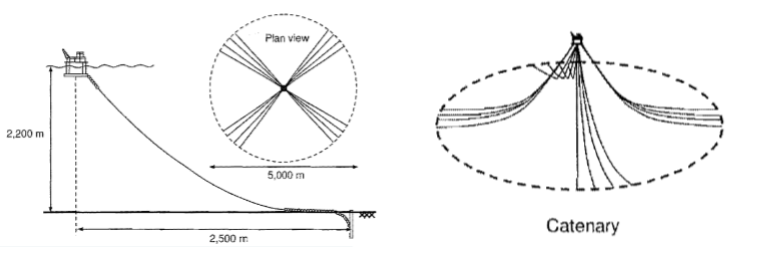
\includegraphics[width=\linewidth]{pictures/part4/photo1.PNG}
\end{center} 

Il s'agit d'un amarre qui prend une forme de caténaire entre l'installation marine et le fond, avec un atterrissage en amont de l'ancrage. La force transmise au sol est donc purement horizontale. L'ancrage est à une distance horizontale d'une ou deux fois la profondeur d'eau. La force fournie par l'ancrage provient principalement du poids de la "corde", l'ancrage lui même ne reprend qu'une fraction infime. Il faut en placer entre 8 et 16 pour que ce soit efficace. La partie en contacte avec le sol est une chaîne, pour augmenter les frottements.

\subsection{Taut or semi-taut line moorings}

\begin{center}
    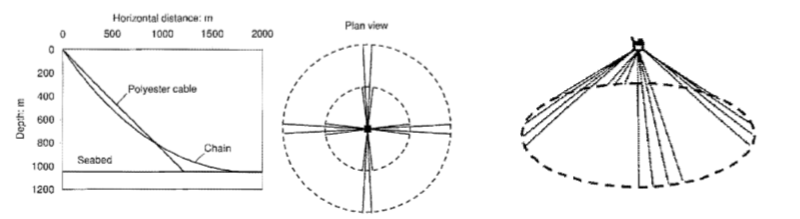
\includegraphics[width=\linewidth]{pictures/part4/photo2.PNG}
\end{center} 

Utile pour les eaux très profondes, les amarres caténaire seraient beaucoup trop lourd. Elles sont plus légère et dimensionnée pour arriver à un angle précis, la résistance est transmisse aux fonds marin par l'élasticité de l'amarre. Il y a donc des forces verticales et horizontales. La dimension de la base est réduite par rapport aux précédente, environ 1x la profondeur (angle de 30\degree ou 45\degree). On utilise le même nombre d'amarres.

\subsection{Vertical line moorings}

Utilsé pour les TLP. importance de la composante cyclique (due au vague) transmise au sol. Effort essentiellement vertical. Peut être utilisé pour de grande profondeur (>150m). très petite emprunte au sol. On utilise des câbles car il y a beaucoup de tension, on utilise toujours entre 8 et 16 lignes.

\section{Types of anchors}

\subsection{Surface gravity anchors}

En gros un bloc très lourd de béton qui retiens l'amarre par son poids propre. Prend vite beaucoup de place et on le limite au eau peu profonde. On rajoute parfois des pieux sous le poids pour augmenter la force de friction.

\subsection{Embedded anchors}

Crée une cassure plus profonde dans le sol. La capacité va dépendre de la résistance du sol. La ligne d'amarre utilisé va aussi être prise en compte dans la capacité totale. Il en existes trois grands types : 
\begin{itemize}
    \item Anchor piles
    \item Suction caissons
    \item Drag anchors
\end{itemize}

\subsubsection{Anchor piles}

Tube creux installé par forage (driving or drilling \& grouting). Long et fin, ils peuvent supporter des forces verticales et horizontales. Installé profondément (150m) avec de grand diamètre (1 à 2.5m), ils peuvent supporter de très grandes charges. "The anchor chain is either fixed at a padeye some height along the pile length or grouted into the top pile assembly. This affects the relative horizontal/vertical capacity but also the location of potential plastic points and failure modes."

\subsubsection{Suction caisson anchors}

Diamètre plus grand que les anchor piles (3 à 8m) mais longeurs plus petite (3 à 6m). On renforce l'intérieur pour éviter le flambement et augmenter la résistance du caison à l'endroit de l'ancrage. 

\begin{center}
    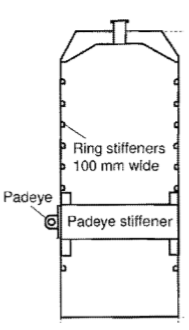
\includegraphics[scale=1]{pictures/part4/photo3.PNG}
\end{center} 

Le caisson pénètre d'abord le sol grâce à sont poids propre, le reste est effectué par succion de l'eau dans la "jupe". La force verticale acceptable est alors une combinaison entre la force de succion et les frottement de la jupe contre le sol. La capacité horizontale est optimal pour un amarre enfoncé à 60-70\% de la profondeur du caisson.

\subsubsection{Drag anchors}

Évolution de l'ancre traditionnelle utilisée sur les bateaux, Comprend trois parties : un fluke, un shank et le padeye.

\begin{center}
    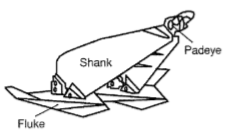
\includegraphics[scale=1]{pictures/part4/photo4.PNG}
\end{center} 

l'angle est prédéterminé pour optimiser la résistance (50 degrés pour les argiles molles et 30 degrés pour les sables). La pénétration s'obtient en draguant l'ancre le long du sol. Il faut atteindre une profondeur de 1 à 5 fois la taille du fluke, ce qui représente une distance de dragage de 10 à 20 fois la longueur du fluke. Pendant la pénétration, l'angle est réduit pour facilité la pénétration. Une fois la position finale obtenue, la ligne d'ancrage est tournée perpendiculairement au fluke pour augmenter la capacité de résistance (20-50 fois le poids de l'ancrage). On peut la retirer facilement en faisant la démarche arrière.

\subsubsection{SEPLA anchors (suction embedded plate anchor)}

En gros, on enfonce une drag anchors grace une force verticale fournie par succion. Il ne faut plus dragger. Peut être enfonc jusqu'à 25m.

\subsubsection{Dynamically-penetrating anchors}

Facile à construire (pas cher) et facile à mettre en place, elle s'enfonce grâce à sa vitesse (environ 30 m/s). Le problème est que ce n'est pas efficace en sol dur. Si on arrive à pénétrer profondément, on peut obtenir une capacité de 3 à 6 fois le poids de l'ancre.

\section{Design of gravity anchors}

\underline{Drained :}

Frottement mobilisé à la base, on utilise des ratios de contrainte de cisaillement de 0.5, 0.7, On ne considère pas les charges cycliques car elles ne changent pas de direction. Il peut en résulter un petit déplacement et une réduction de l'angle de friction, on prend donc un ration de 0.3 pour la contrainte de cisaillement. 

\underline{Undrained :}

On considère la limite plastique du matériel qui risque d'arriver pour une pression de 6 à 12 fois la force de cisaillement de base. Toutefois, on considère une force de cisaillement maximale de 1/3.

\section{Profile of an embedded anchor line (catenary mooring}

La tension horizontale de la ligne d'ancrage provoquera le glissement de la chaîne dans le sol. La chaîne adopte un profil caténaire inverse et participe à la capacité de rétention. L'angle de la chaîne augmente avec la profondeur, transférant ainsi une force verticale.

\begin{center}
    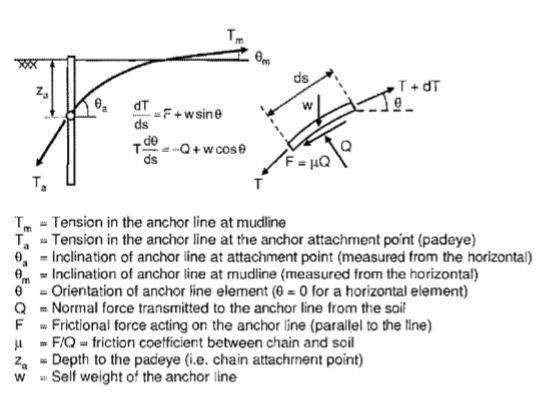
\includegraphics[scale=1]{pictures/part4/photo5.PNG}
\end{center} 

La capacité portante résulte d'une égalité de force :

\begin{itemize}
    \item La force de friction : $ F = A_s \alpha s_u $ avec $A_s = \pi d$, et $\alpha$ le coefficient de friction $=0.2 - 0.60$.
    \item la force maximale : $ Q = A_b N_c s_u $ avec $A_d=2.5$ pour une chaîne et =d pour un câble et avec $N_c=7.6$ pour une "buried strip footing".
\end{itemize}

On obtient : 
$$ \theta_a = \sqrt{\frac{2Z_a Q_{av}}{T_a}} $$
$$ \frac{T_a}{2}(\theta_a^2 - \theta_m^2) = z_a Q_{av}$$
$$ z_{a_{av}} = bN_c \int^{z_a}_0 s_u dz$$

\section{Design principle of drag anchor}

On peu se baser sur les designs existant dans le commerce. La capacité portante étant plus lié au dimension de l'ancre plutôt qu'au poids, on peu se baser sur la géométrie.

La résistance à la pénétration d'un ancrage est : $T_p = (fA_p)N_cS_u$ avec $A_p$ la surface frontale et $N_c = 9$, un facteur de la capacité portante et f un facteur de forme. On peut l'exprimer en fonction de l'angle $\beta$ tout au long de son enfoncement, jusqu'a ce que $\beta = 0$ à la position finale. On obtiendra : 
$$ T_a = \frac{T_p}{cos \theta'_w}  \frac{fA_p N_c s_u}{cos \theta'_w}$$

qui agit selon l'angle : 

$$ \theta'_w = tan^{-1} \frac{W + T_p tan \theta_w}{T_p} $$

\section{Design principle of a suction caisson}

La résistance à la pénétration provient de :
\begin{itemize}
    \item La contrainte de cisaillement le long de la jupe : $Q = A_s \alpha s_u$
    \item La capacité portante du sol : $Q = A_{tip} N_c s_u$
    \item la surpression du sol : $Q = A_{tip} \gamma' z$
\end{itemize}

En métant tout ensemble, on obtient : $$ Q = A_s \alpha s_u + A_{tip} (N_c s_u + \gamma'z)$$

\begin{center}
    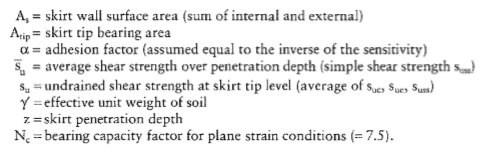
\includegraphics[scale=1]{pictures/part4/photo6.PNG}
\end{center} 

\begin{center}
    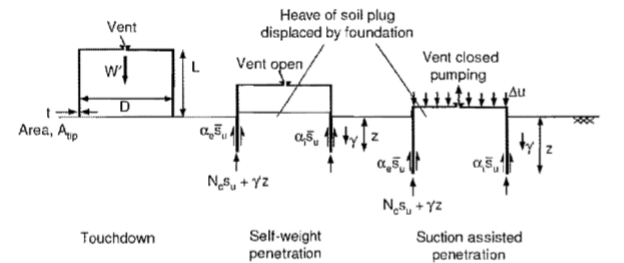
\includegraphics[scale=1]{pictures/part4/photo7.PNG}
\end{center} 

La succion minimum permettant la pénétration est : 

\begin{center}
\begin{tabular}{c|c}
    $\Delta u_{req} = \frac{Q - W'}{A_i} $ &   Q = total penetration resistance  \\
                                           &  W' = Submerged weight of foundation   \\
                                           &  $A_i$ = la section internet  
\end{tabular}
\end{center} 

La succion maximale qui causerai une cassure dans le sol est :

$$\Delta u_{a} = \frac{A N_c sU + A_{si}\alpha s_u + W'_{plug} - \gamma' d A_{plug}}{A_i} $$ 

\begin{center}
    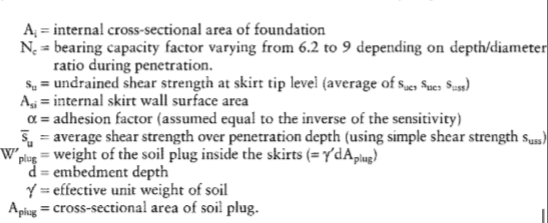
\includegraphics[scale=1]{pictures/part4/photo8.PNG}
\end{center} 

\underline{La capacité portante verticale :}

\begin{center}
    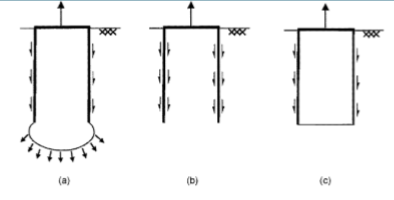
\includegraphics[scale=1]{pictures/part4/photo9.PNG}
\end{center} 
\begin{itemize}
    \item a) Avec "reverse end bearing and external shaft resistance : $ V_{ult} = W' + A_{se} \alpha_0 s_{u(t)}+N_cs_uA_c$.
    \item b) Witauut passive suction : $V_{ult} = W'+A_{se}\alpha_0 s_{u(t)} + A_{si}\alpha_i s_{u(t)}$.
    \item c) Witauut passive suction but with simultaneous pullout of soil plug : $V_{ult} = W' + A_{se} \alpha_es_u(t) + W'_{plug}$
\end{itemize}

\underline{La capacité portante horizontale :}
Elle est maximum

\begin{center}
\begin{tabular}{c|c}
    $H_{max} = L D_e N_p s_u$ &  L = embedded length of the caisson  \\
                              &  $D_e$ = external diameter of caisson  \\
                              &  $N_p$ = lateral bearing capacity factor  \\
                              &  $s_u$ = average undrainded shear strength 
\end{tabular}
\end{center} 

Les rupture du sol des forces horizontale implique une rupture de coin conique et une rupture d'écoulement confiné sous le coin. 

\begin{center}
    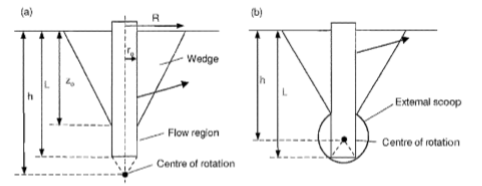
\includegraphics[scale=1]{pictures/part4/photo10.PNG}
\end{center} 

\section{Jack-up rigs and spudcans: overview}

\subsection{installation}

\begin{itemize}
    \item amené sur place avec les jambes levé
    \item On descend les jambes jusqu'au fond (environ 1 m/h)
    \item On précharge en pompant l'eau de mer sur la plate-forme
    \item On remonte la plate-forme pour être à l'abri des vagues.
\end{itemize} 

\begin{center}
    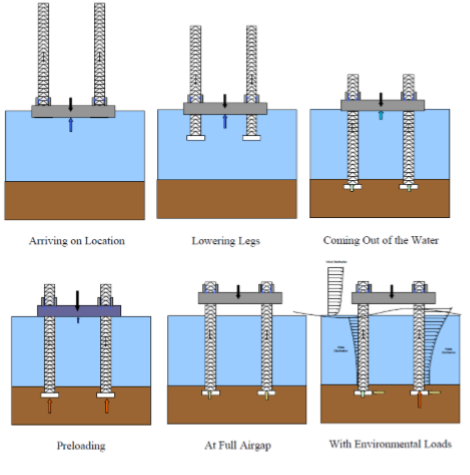
\includegraphics[scale=1]{pictures/part4/photo11.PNG}
\end{center} 

\subsection{risques}

Punch throught (31\% + 14\%) / rapid penetration, foundation failure, boulders, liquefaction, ...

Vertical resistance in UNDRAINED conditions and homogenous soils :
On se base sur l'équation de la portance classique : $V = A (s_u N_c + \sigma'_{v0})$. La force de cisaillement est moyenne à partir d'une profondeur valant D/2. Pour les faibles pénétration, la capacité portante est fonction de la profondeur et du type de rupture possible.

Il faut faire attention, au dessus d'une certaine profondeur, il y a un risque de remplissage par dessus de la fondation qui empire la pénétration. 

Pour les pénétration profonde, on considère la formule finale :
$$ V = s_uN_{cd}A+\gamma'V_{spudcan}$$ 

avec $N_{cd} = 10(1+0.065 \frac{w}{D})<11.3$.

Vertical resistance in DRAINED conditions (sand) and homogeneous soils :
On se base également sur l'équation de la portance: 
$$ V =\gamma' N_{\gamma} \pi \frac{D^3}{8} $$ 

Ces déformations sont généralement petite au point que parfois la totalité de la surface ne touche même pas le sol. 

\begin{center}
    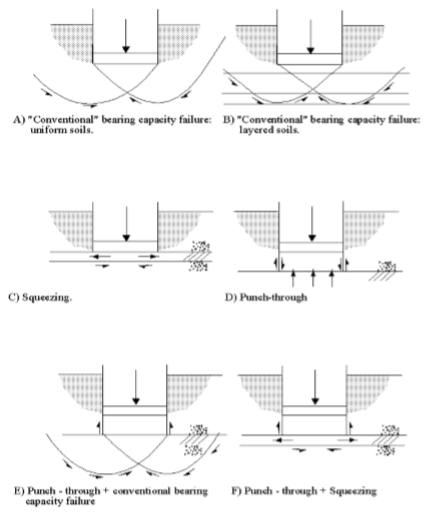
\includegraphics[scale=1]{pictures/part4/photo12.PNG}
\end{center} 

\subsubsection{Squeezing failure}

Arrive si $T<\frac{1}{3} B$, la résistance ne peu devenir plus grande que la résistance de la couche inférieur.
\begin{center}
    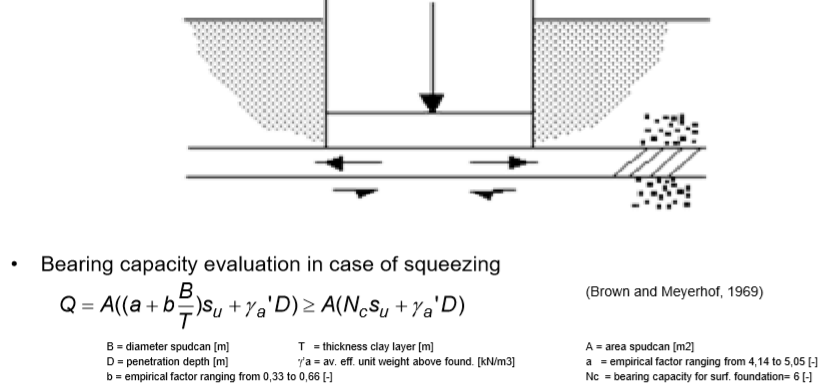
\includegraphics[width=\linewidth]{pictures/part4/photo13.PNG}
\end{center} 

\subsubsection{Punch through}

\begin{center}
    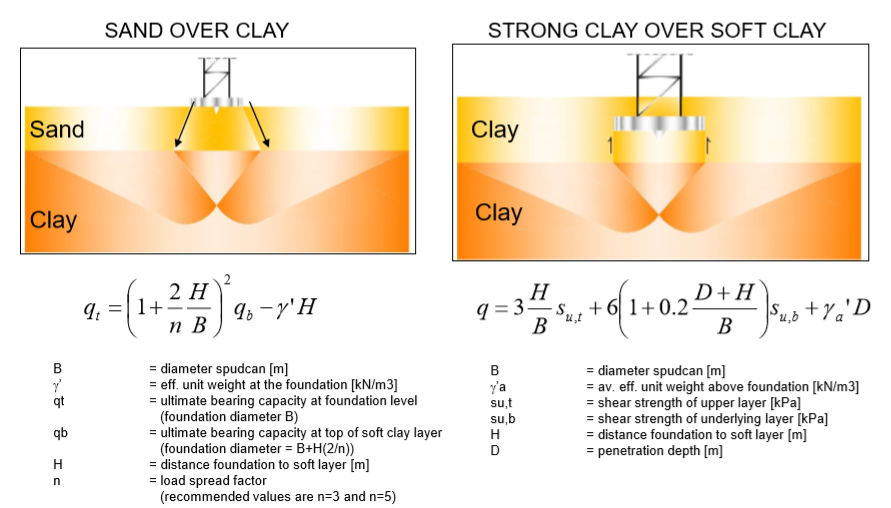
\includegraphics[width=\linewidth]{pictures/part4/photo14.PNG}
\end{center} 

\begin{center}
    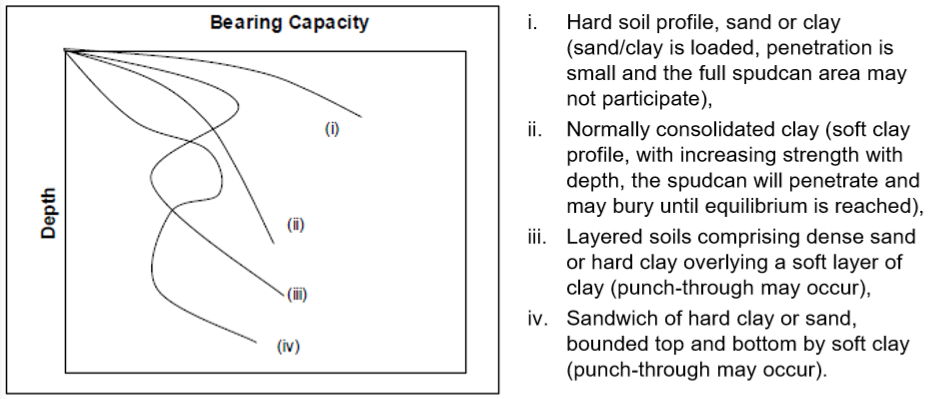
\includegraphics[scale=0.8]{pictures/part4/photo15.PNG}
\end{center} 

\subsubsection{Résumé}

Il y a trois évènement qui peuvent se produire lors de l'enfoncement d'un spudcan :
\begin{itemize}
    \item Backflow : si le trou est trop profond, le sol se déverse dedans
    \item Squeeze : si $T<1/3 B$ le sol se défausse latéralement 
    \item Punch trough : grande perte de résistance, la force pousse les particules à travers la couche suivante.
\end{itemize}

\subsubsection{Extraction de la spudcans}

\begin{center}
    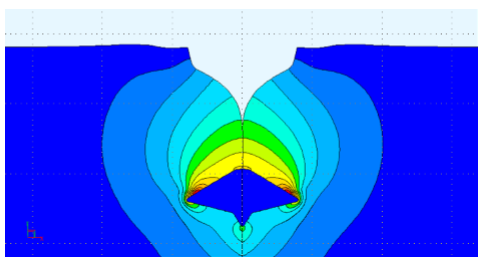
\includegraphics[scale=0.8]{pictures/part4/photo16.PNG}
\end{center} 

La résistance à l'extraction est du au remblais formé par déversement des côtés (backflow). Certain on pu se reconsolidé durant le déploiement de la spudcan. Cette force est bien moindre que la résistance verticale de la fondation. La barge ne peut appliquer que 20 à 50\% de la force qu'elle peut déployer lors de l'installation.

Ca représente un défit à cause  d'un important phénomène de succion (surtout avec des argiles rigide) à la base. On peut alors l'équiper de buse à jet d'eau qui visent à supprimer la sous-pression pendant l'extraction (Cela fonctionne moyennement).

\newpage
\part{Lecture 5 ??????}

Aucune info ! (20-04-2018)

\newpage
\part{Cyclic Loading}

Les informations ci-dessous sont basées sur le chapitre 4.2 du livre "Offshore Geotechnical Engineering".

\section{introduction}

Souvent du à des forces environnemental (courant, vent, vague, séisme,...) , elles affectent surtout les fondations, pipelines/câbles, ou les zones proches des côtes (port, pontons, ...).

Les charges cycliques génèrent un excès de pression interstitielle, réduisant ainsi les contraintes effectives dans les fonds marins. Des forces de cisaillement se développent causant une perte de résistance au cisaillement ou de rigidité des sédiments marins.

Change la rigidité et la force du sol à cause d'actions répétée (micro-structure altérée). Ne conduit pas toujours à des dégradations. 

La réponse du sol est très différentes face à des charges ponctuelles, constantes ou cycliques. Le type de sol influençant peu dans bien des aspects, il est possible d'approcher le problème cyclique de manière unifiée. Les réponses dépendent du mode, de l'amplitude et de la fréquence du cycle de chargement. Il faudra néanmoins différencier sable et argile.
\begin{itemize}
    \item Sable : possible liquéfaction,
    \item Argile : possible perte de résistance au cisaillement non drainée, création de pression interstitielle et sa perte subséquente et une accumulation de déformations permanentes.
\end{itemize}

\section{Comportement du sol sous un chargement cyclique}

La rigidité n'est pas linéaire :

\begin{center}
    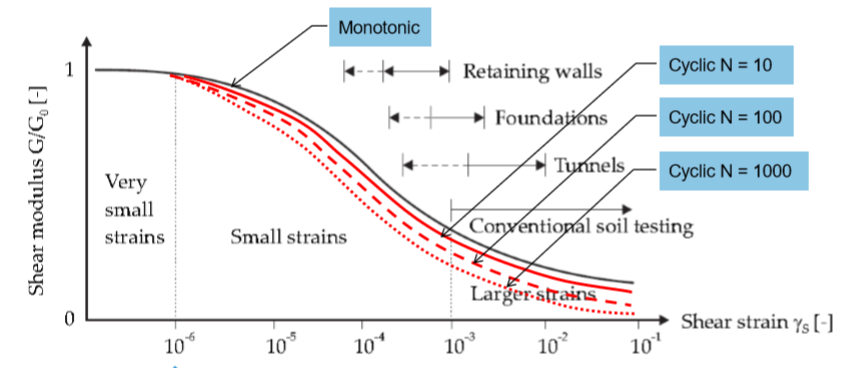
\includegraphics[scale=0.8]{pictures/part6/photo8.PNG}
\end{center} 

On remarques deux comportements : Dynamique (comportement linéaire élastique) et Cyclique (comportement non linéaire plastique). Dans le deuxième il y a une dégradation du degré de rigidité et une accumulation des contraintes permanentes.

Une accumulation des déformations plastiques induit une dégradation de la rigidité et donc un déchargement du module de rigidité.

\begin{center}
    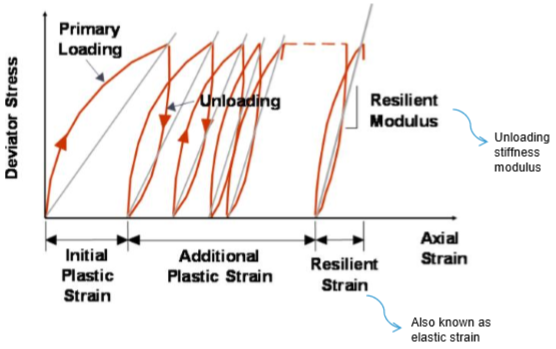
\includegraphics[scale=0.8]{pictures/part6/photo9.PNG}
\end{center} 

\underline{Hysteresis Damping $\lambda$ :} "effet ammortisseur"
$$\lambda_N = \frac{1}{2\pi}\frac{\Delta E}{G_{s,N}\gamma_{c,N}^2}$$

\subsection{Shakedown theorem de la plastoméchanique}

\begin{itemize}
    \item Cas 1 : Purement élastique : Déformation cyclique suffisamment faible, il n'y a pas de déformation plastique.
    \item Cas 2 : Rupture ordinaire : Déformation cyclique suffisamment importante, les ruptures interviennent instantanément. Développement de déformations plastiques spontanées.
    \item Cas 3 : Rupture grandissante : La charge cyclique n'est pas suffisante, accumulation de déformations plastiques. Elles deviennent trop importante et dépasse la limite de service.
    \item Cas 4 : Extorsion (Shakedown) ou Adaptation : Sous de faibles charge cyclique, une déformation plastique apparaît mais se stabilise après un nombre fini de déformation
\end{itemize}

\begin{center}
    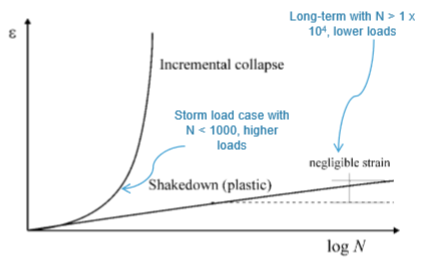
\includegraphics[scale=0.8]{pictures/part6/photo10.PNG}
\end{center} 

\section{Le mode de chargement cyclique}

Bien que dans les faits, la fréquence et l'amplitude sont irrégulier, en laboratoire on test avec des valeurs constantes.

\begin{itemize}
    \item $\tau_{cy}$ : amplitude de l'effort cyclique,
    \item $\tau_a$ : effort moyen appliqué durant le cycle.
\end{itemize}

\section{Test de chargement cyclique}

Il faut essayer de refléter au mieux les efforts rencontré in-situ. On utilise généralement une fréquence de 0.05 à 0.1 Hz (représente la fréquence des vagues). Des essais triaxiaux ou de cisaillement simple sont couramment réalisés bien qu'il soit de plus en plus courant de centrer les essais cycliques sur de simples essais de cisaillement (moins de matos, moins cher).

\section{Interprétation des données}

\underline{rappel :}
$$ \sigma = \sigma' + u $$

\subsection{Essai de cisaillement simple monotone sur fond marin sableux}

Dans la phase de cisaillement, on maintient la contrainte verticale ($\sigma_v$) constante et on applique un cisaillement. Initialement, l'échantillon se contracte et un excès de pression interstitielle ($u_e$) est produit, ce qui produit une diminution de la contrainte effective verticale ($\sigma_v'$). Une foi le maximum atteint, la pression interstitielle décroît indiquant une dilatation et une augmentation de la contrainte effective. Le point de passage entre contraction et dilatation est appelé phase de transformation (PT).

\begin{center}
    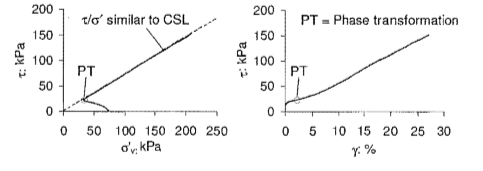
\includegraphics[scale=0.8]{pictures/part6/photo1.PNG}
\end{center} 

Une fois la transformation passée, le chemin de contrainte se déroule de manière relativement constant ($\tau/\sigma'$). Ce chemin est parfois appelé "Critical State Line" (CSL). Mais ce n'est pas tout à fait vrai, il s'agit en réalité juste de sa projection dans le repère ($\tau, \sigma'$).

Si on avait continué le test jusqu'à ce que l'excès de pression interstitielle se stabilise alors on aurait atteint un état critique (déformation à effort et volume constant). On observe une réponse rigide durant la phase initiale de cisaillement (Module de cisaillement G = $d\tau/d\gamma$) suivie d'une réponse plus douce (gradient presque constant) à l'approche de la phase de transformation.

\subsection{Essai de cisaillement simple cyclique sur fond marin sableux}

Comme précédemment, on maintient la contrainte verticale constante pour observer une variation de la pression interstitielle et de la contrainte verticale effective.

\begin{center}
    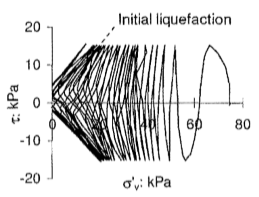
\includegraphics[scale=0.8]{pictures/part6/photo2.PNG}
\end{center} 

La première partie du graphe correspond au test monotone. Un excès de pression interstitielle est généré durant la contraction de l'échantillon ce qui provoque une réduction de la contrainte effective. L'excès de pression continue à augmenter avec chaque cycle de chargement (à l'inverse du test monotone). Finalement, l'excès de pression interstitielle (au "mid-point" de chaque cycle) atteint $\sigma_v$. On a donc une contrainte effective verticale nulle. La première fois que ce phénomène est atteint est appelé liquéfaction initiale. Une fois que ce point est atteint, l'échantillon tend à se dilater (avec une réduction de pression interstitielle) (ce qui donne explique cette forme de graphique en S).

\begin{center}
    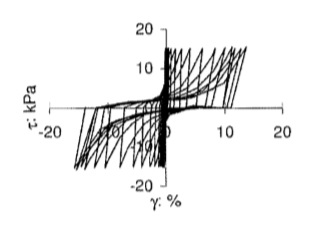
\includegraphics[scale=0.8]{pictures/part6/photo3.PNG}
\end{center} 

La rupture n'intervient pas spécialement au début de la liquéfaction. Ça reste néanmoins intéressant d'avoir une idée de l'effort de cisaillement nécessaire pour liquéfier le sol. 
Une contrainte de cisaillement de 15\% est généralement adaptée bien qu'une limite de service peu être établie plus base.

On observe initialement une accumulation très lente de l'effort de cisaillement, mais une fois qu'il y a liquéfaction, l'effort de cisaillement grandit et la rigidité réduit rapidement.

\subsubsection{Effet d'un effort de cisaillement cyclique $\tau_{cy}$}

\begin{center}
    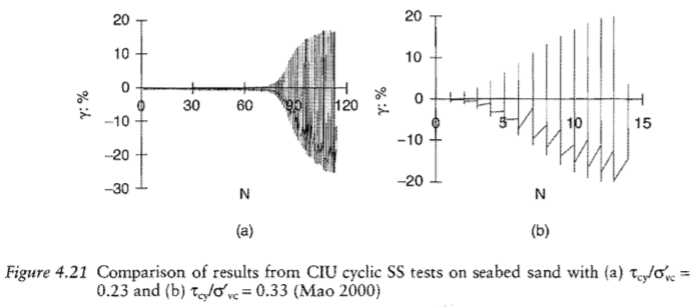
\includegraphics[scale=0.8]{pictures/part6/photo4.PNG}
\end{center} 

La réponse générale est la même, un excès de pression interstitielle qui grandit rapidement initialement, atteint finalement  la contrainte verticale et donc le point de liquéfaction. L'effort de cisaillement augmente initialement lentement jusqu'à ce que le sol perde sa rigidité (liquéfaction) pour ensuite augmenter rapidement. La différence entre les deux tests est le nombre de cycle avant d'atteindre une rupture (a environ 100 alors que seulement une dizaine pour b).

\section{Courbes de résistance cyclique}

Les courbes de résistance cyclique sont utilisées pour définir la contrainte de cisaillement cyclique $\tau_{cy}$ pour atteindre une valeur donnée de déformation de cisaillement après un certain nombre de cycles N. On peu utiliser les résultats des essais vu précédemment pour construire ces courbes.

\subsection{Diagrammes de contours des déformations}

\begin{center}
    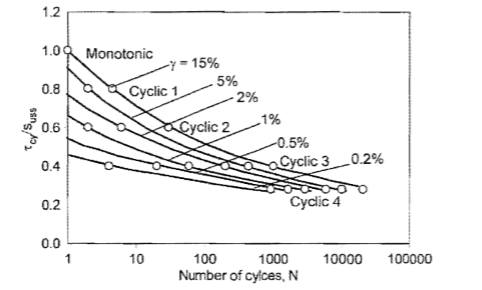
\includegraphics[scale=0.8]{pictures/part6/photo5.PNG}
\end{center} 

\subsection{Diagrammes de contours des pressions interstitielles}

L'amplitude des pressions d'eau interstitielle en excès générées sous chargement cyclique peut être exprimée en fonction du nombre de cycles de chargement.

\begin{center}
    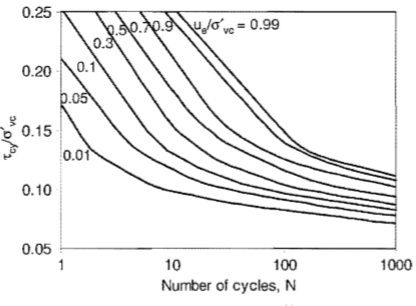
\includegraphics[scale=0.8]{pictures/part6/photo6.PNG}
\end{center} 

\subsection{Fugro Soil Cyclic Database - Undrained}

La fonction d'interpolation donne la résistance et la déformation du sol pour un CSR donné, le nombre de cycles et la densité du sol pour le sable ou la consistance pour l'argile

\underline{Argile :}
\begin{center}
\begin{tabular}{c|c}
$CSR = \frac{\tau_{cyc}}{S_u}=a.exp(b\frac{S_u}{\sigma'_{vo}})+c \le 1 $
        &  a,b et c: empirical parameter 
\end{tabular}
\end{center}

\underline{Sable :}
\begin{center}
\begin{tabular}{c|c}
$CSR = \frac{\tau_{cyc}}{S_u}=A(\frac{S_u}{\sigma'_{vo}}+B)^C$
        &  A,B et C: empirical parameter 
\end{tabular}
\end{center}

\begin{center}
    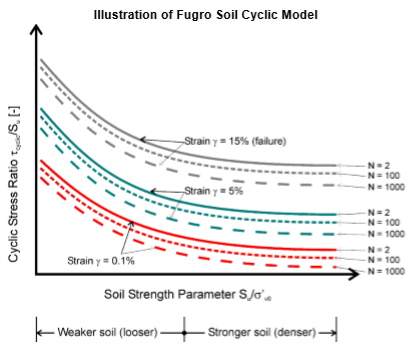
\includegraphics[scale=0.8]{pictures/part6/photo11.PNG}
\end{center} 

\subsection{Irregular cyclic load histories}

Plutôt que de modéliser la séquence de chargement complète, la conception offshore utilise souvent un nombre «équivalent» de cycles de la charge de pointe pour représenter les dommages cumulatifs qui se produisent sous la séquence complète. Soit le diagramme de déformation de cisaillement ou de contour de pression interstitielle en excès peut former la base pour établir le nombre équivalent de cycles.

\begin{center}
    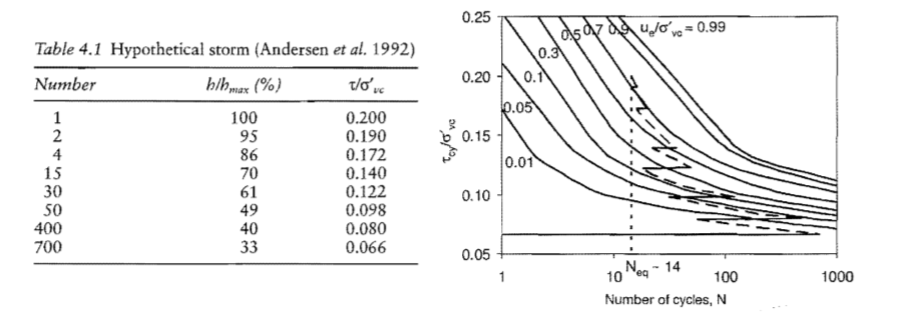
\includegraphics[width=\linewidth]{pictures/part6/photo7.PNG}
\end{center} 

\underline{méthode :}
On part du plus petit niveau de chargement, qu'on place dans le graphe, on reviens parallèlement au contour le plus proche pour atteindre le prochain cycle d'effort de cisaillement de la tempête. Le point obtenu représente le même niveau de dégât obtenu par le cycle du niveau précédent. On répète le process en repartant du point obtenu (donc on rajoute le nombre de cycle à celui du point sur lequel on se trouve). Le processus ce termine avec le nombre de cycle équivalent pour ce chargement précis (généralement N = 10-20).

\subsection{Construction d'une courbe de contrainte déformation}

Voir 4.2.7 p 167 du pdf ou 137 du bouquin

\subsection{Chargement cyclique non symétrique}

En réalité, les conditions de contrainte dans le sol sous les structures soumises à des combinaisons de charges statiques et cycliques sont plus complexes et l'effet du niveau de contrainte de cisaillement moyenne sur la réponse à la charge cyclique doit être considéré.

\subsection{Mécanismes de rupture}

Le sol n'aura pas toujours le même comportement. Cela dépendra du type de sol, de sa géométrie, de l'amplitude de la charge, de la fréquence, ... Le "stress-path" dépendra de la rigidité du sol et de sa force.

\begin{center}
    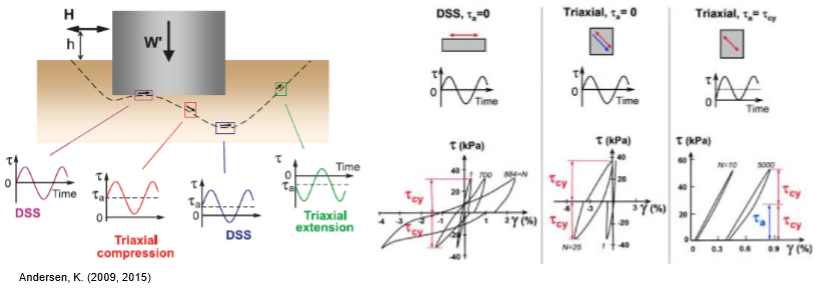
\includegraphics[scale=0.8]{pictures/part6/photo12.PNG}
\end{center} 

Il faudra prendre en compte différents aspects, sur un même "stress-path" on peut croiser différent cas de charge : 

\begin{center}
    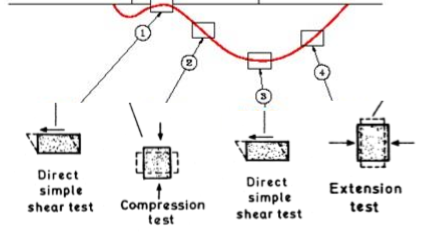
\includegraphics[scale=0.8]{pictures/part6/photo13.PNG}
\end{center} 

\section{méthode pour déterminer le module de cisaillement ($G_0$)}

On émet des ondes sonores polarisée horizontalement et qui se propagent verticalement dans le sol. On peut récupérer cette onde de deux manières : 
\begin{itemize}
    \item par un géophone placée dans un forage (il est alors possible de faire un forage annexe et de directement placer une source sonore à même auteur que le géophone (cette fois l'onde se propage horizontalement et est donc polarisée verticalement))
    \item Par un oscilloscope relié à un cône sismique ou un dilatomètre (pénétration test).
\end{itemize}

L'avantage de la méthode par forage est qu'on peut récupérer une carotte et ainsi connaître le module par des test en laboratoire.

On utilise alors trois tests :

\subsection{Bender Element Test}

On place l'échantillon entre des blaques Piezo-electrique qui vont se courber à cause d'un voltage appliqué. L'échantillon va également générer un voltage en se courbant. On détermine $G_0$ grâce à la vitesse de l'onde de cisaillement récupérée.

\begin{center}
    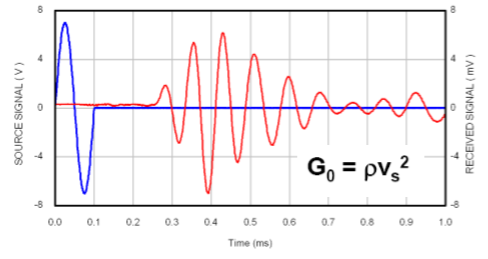
\includegraphics[scale=0.8]{pictures/part6/photo14.PNG}
\end{center} 

L'essai à été améliorer par Pennington en 1997 en rajoutant des émetteur. On peut donc produire des ondes de cisaillement verticalement ou horizontalement.

\subsection{Resonant column test}

 On applique une torsion au cylindre récolté par forage. On connaît la fréquence de résonance en mesurant le mouvement du côté non fixé. La vitesse de l'onde de cisaillement peut être ainsi déterminé en utilisant une solution élastique (c'est évident !). Et comme avant on connait G grâce à la formule :
 $$ G = \rho v_s^2 $$ 
 
 \begin{center}
    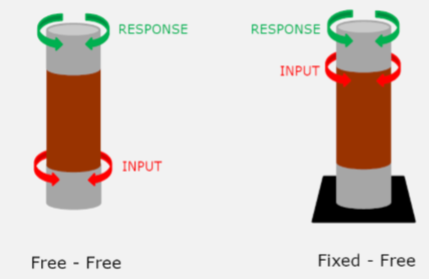
\includegraphics[scale=0.8]{pictures/part6/photo15.PNG}
\end{center} 
 
 \subsection{Cyclic Triaxial Test}
 
 On applique une charge triaxial cyclique. On mesure  le cisaillement et la résistance au cisaillement durant l'essai. On dresse un graphe et on en déduit G, le module de cisaillement.
 
  \begin{center}
    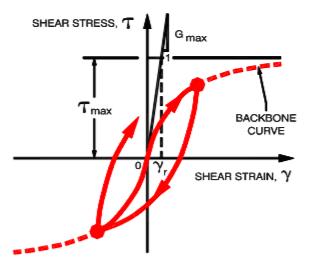
\includegraphics[scale=0.8]{pictures/part6/photo16.PNG}
\end{center} 

\section{Fondation en eau peu profonde (250m)}

Utilisation de Donut foundation avec robe pour les RSS avec des tanks de flottabilité temporaires.

\subsection{Considérations de dimensionnement}

Des couches de sol très fines peuvent être critique pour la stabilité, le sol va subir différent type d'efforts : compression vertical, cisaillement, compression horizontale,... Il faut teste la dégradation due aux efforts cycliques. Les tassements peuvent être critique, la robe doit s'enfoncer suffisamment pour être efficace et le sol doit être suffisamment résistant pour tenir les chargements durant les tempêtes.

\subsubsection{Capacité portante ultime}

\begin{itemize}
    \item Chargement : combinaison de plusieurs charge
    \item Mechanisme de rupture (ULS) :
    \begin{itemize}
        \item glissement (translation horizontale)
        \item portance (translation verticale)
        \item Rotation
        \item Mixe : translation et rotation, translation et torsion, ...
    \end{itemize}
\end{itemize}

\subsubsection{Tassements}

Ils doivent être uniforme et prévisible. Pour ca une investigation du site est vital ainsi que tester la dégradation sous charge répétée et tester plusieurs mode de rupture possible.

\subsubsection{Gravity Base Structure}

Il n'y a plus aucune logique dans l'ordre de ces putains de slides !!!! je sais pas ce que ca fou ici :p 

\underline{Avantages :}

prix peu cher et relativement fixe, ne produit pas de bruit, construction onshore ce qui limite les risques, capacité connue et maîtrisée, prix de maintenance bas et complètement remplaçable/enlevable.

\underline{Désavantages :}

Applicable qu'entre 20 et 40m, dépend fortement des conditions de fond marin, il faut prendre en compte la protection du sol et sa préparation et cela nécessite une bonne connaissance des propriétés géotechniques et des conditions requissent.

\subsubsection{Wind Turbines}

On utilise souvent des gravity base (ca doit être pour ca que c'est ici !). Génère énormément d'efforts cyclique à cause du vent (grandes forces horizontales). Des tests statiques risquent de ne pas prendre en compte la rigidité du sol et donc de ne pas bien dimensionner le système. Les fréquences peuvent atteindre 0.1 à 0.5 Hz.

Il faut prendre en compte qu'un effort de torsion peut diminuer l'effort de portance localement. Il y a des risques de mouvement verticaux de la fondation ayant pour conséquence un effet de pompe sur les fonds marins. Il faut donc une préparation ou une jupe. 

Il faut prendre compte du temps de consolidation (pore pressure dissipation) pour estimer le gain en capacité portante du sol. Il existe maintenant des softwares qui calcule la capacité portante du sol pour différentes combinaisons de charges.

\subsubsection{Capacity analysis - ULS}

Permet un dimensionnement rapide d'une fondation sujette à des charges constantes et cycliques. 
Elle prend en compte la force cyclique du sol ($S_u$):
\begin{itemize}
    \item Basé sur les résultats des tests monotones et cycliques du sol,
    \item Prise en compte de la force monotone qui augmentent avec la consolidation (sous le poids statique de base),
    \item Prise en compte de la dégradation de la résistance cyclique et des différents CLR,
    \item Procédure itérative pour diverses combinaisons de V et H pour une variété de CLR.
\end{itemize}

\newpage

\part{Piled Foundations}

(pas vu en cours donc juste comprendre vaguement les notions)

\section{considérations Générales}

\subsection{Loads on piles for offshore structures}

\begin{itemize}
    \item Poids de la structure (axial)
    \item Vent  (latéral et cyclique)
    \item Vagues (latéral (la plus importante) et cyclique)
    \item Collisions avec un bateau (latéral et dynamique)
    \item Tremblement de terre
\end{itemize}

\subsection{Deep pile foundations vs shallow foundations}

Sol mou en surface avec de grandes charges verticales, abîme fonds marins. Il peut y avoir un tassement important et les fondations profondes on une meilleure résistance aux charges horizontales. Plus grand risque de "Scour" pour les fondations peu profondes.

\subsection{Typical features}

Tube en acier, grande capacité axiale (80 MN environ 8000 tons), diamètre de 0.76 à 5m (30 to 200 inch). Épaisseur typique (D/t) = 1/30 - 1/60. Installation jusqu'à 150m de profondeur. Reprend de la pression et de la compression.

Ils sont généralement installé par poussée mais peuvent être foré et jointé (sédiment calcaire ou roche), poussé et jointé (expérimental) ou vibré et frappé (windfarms). La mode est d'utiliser des diamètre de pieux plus large et d'utiliser un marteau hydraulique sous l'eau.

\subsubsection{Driven piles}

\begin{center}
    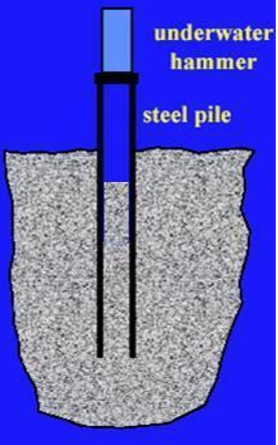
\includegraphics[scale=0.8]{pictures/part7/photo1.PNG}
\end{center} 

Installation : On les pousse à travers un guide jusqu'à une profondeur déterminée.
Problems : Difficile à enfoncer dans les sables dense et les cailloux mous. Efforts de fatigue, bouchage prématuré et on risque de rencontrer des sables calcaire avec une friction faible. Cette mise en place fait du bruit.

\subsection{Drilled and grouted piles}

\begin{center}
    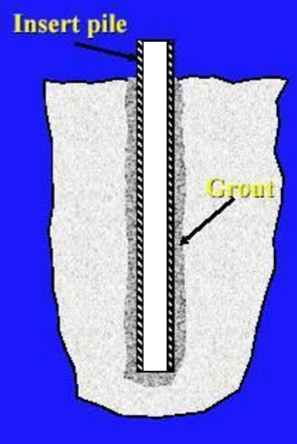
\includegraphics[scale=0.8]{pictures/part7/photo2.PNG}
\end{center} 

Installation : Création d'un trou sur-dimensionné, on installe la fondation et on rempli.
Problems : Stabilité du trou, circulation du "grout", cher, capacité portante ignorée, la pression du sol est limitée,...

\section{Axial Capacity Q}

Se divise en deux catégories : Shaft Capacity ($Q_s$) et Base Capacity ($Q_p$)

\subsection{Unpluged (débranché)}

\begin{center}
    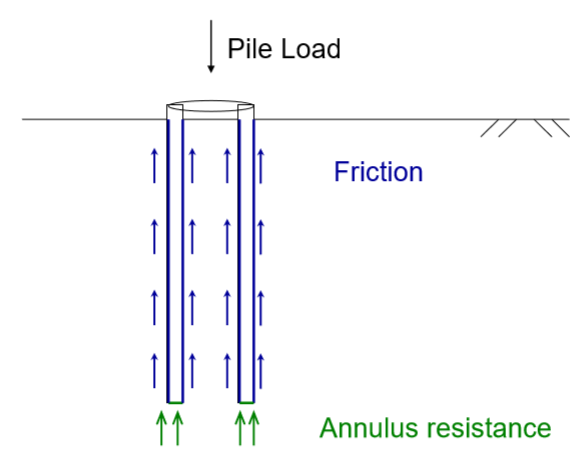
\includegraphics[scale=0.8]{pictures/part7/photo3.PNG}
\end{center} 

Dépend de la friction intérieur et extérieur (Shaft) ainsi que de la résistance de l'anneau (base). La résistance intérieur est plus petite que la résistance possible si on ferme la fondation.

\subsection{Plugged (branché)}

\begin{center}
    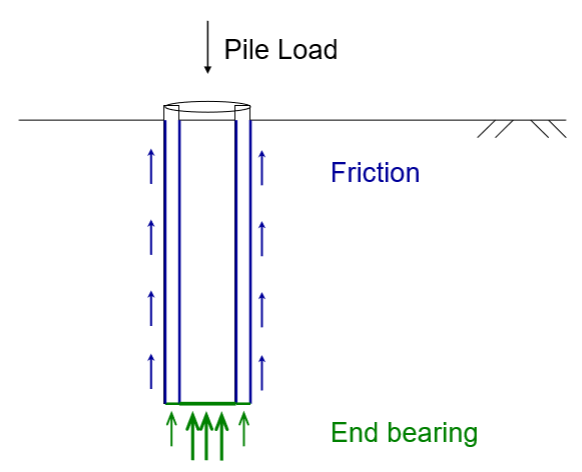
\includegraphics[scale=0.8]{pictures/part7/photo4.PNG}
\end{center} 

Dépend de la friction extérieur et de la section totale. (inner friction > end bearing on plug ?????)

\subsection{Généralité}

Il ne faut pas confondre le cas statique du cas dynamique. Si on l'enfonce entre 2D et 8D, les unplugged deviennent comme plugged.

La capacité axiale est principalement reprise par la base. La résistance le long du puis (shaft) est influencée par les conditions du sol, les contraintes durant l'installation, la rugosité de la fondation, le temps entre l'installation et le chargement et la longueur effective.

\subsubsection{Effet de la longueur}

On a le phénomène de dégradation de la friction, si une fondation devient plus grande, pénètre plus profondément, à une même profondeur on aura moins de friction qu'une fondation plus petite. (API méthode ne prend pas ca en compte, CPT bien ainsi que Kolk \& Van der Velde).

\subsubsection{Résistance}

\begin{center}
\begin{tabular}{c|c}
$F_{shaft} = p \int^{L}_{0} f_z dz$
        &  p: périmètre \\
        &  L: pointe du pieu \\
        &  $f_z$: friction en z 
\end{tabular}
\end{center}

\begin{center}
\begin{tabular}{c|c}
$F_{tip} = A q_z $
        &  A: Aire du pieu \\
        &  $q_z$: portance en z 
\end{tabular}
\end{center}

$$ F_{pile} = F_{shaft} + F_{tip} $$

\subsubsection{méthode API - Argile}

Ne défini pas à partir de combien de temps après l'installation, la capacité calculée est valide.

\begin{center}
\begin{tabular}{c|c c}
$f_z = \alpha c_u$
        &  $\alpha = 0.5 \psi^{-0.5}$  & $\psi \le 1.0$ \\
        &  $\alpha = 0.5 \psi^{-0.25}$  & $\psi > 1.0$ \\
        &  $\psi = c_u / \sigma'_V$  & \\
        &  $\alpha \le 1.0 $  &  
\end{tabular}
\end{center}

\begin{center}
\begin{tabular}{c|c}
$q_z = N_c c_u$
        &  $N_c = 9$
\end{tabular}
\end{center}

\subsubsection{méthode API - Sable}

\begin{center}
\begin{tabular}{c|c}
$f_z = \beta \sigma'_V < f_{lim}$
        &  $\beta$ : dépend de $D_r$ \\
        &  $f_lim$ : dépend de $D_r$ 
\end{tabular}
\end{center}

\begin{center}
\begin{tabular}{c|c}
$q_z = N_q \sigma'_V < q_{lim}$
        &  $N_q$ : dépend de $D_r$ \\
        &  $q_lim$ : dépend de $D_r$ \\
\end{tabular}
\end{center}

\section{Axial Settlement}

Le transfert des charges est simulé par l'emploie de ressorts de différente élasticité (élastique, plastique, non-linéaire avec une réduction de rigidité, ...).

Un pieu subit un tassement lorsqu'on lui applique une charge. Trois composante influence cet effet : 
\begin{itemize}
    \item Développement de la force de frottement (t-z)
    \item Développement de la force de portance à la pointe (q-z)
    \item Diminution de la longueur du pieu (élastique) ($\Delta l$)
\end{itemize}

Le tassement n'est pas très important en offshore contrairement à l'onshore. Mais il est important de comprendre le phénomène. Le pieu ne va pas seulement s'enfoncer mais aussi se raccourcir (en fonction de la rigidité du pieu). Il est important de tenir compte de la friction. 

\subsection{Développement de la force de frottement}

Le comportement du sol peut etre vu comme différents ressorts à différentes hauteur le long du pieu. On peu définir la rigidité de ces ressorts sur base de la courbe t-z aux différentes hauteurs calculée avec API. (t=skin friction)

\begin{center}
    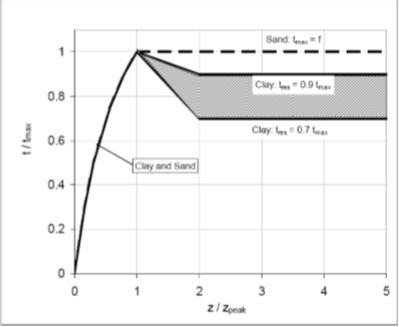
\includegraphics[scale=0.8]{pictures/part7/photo5.PNG}
\end{center} 

\subsection{Développement de la force de portance à la pointe}

Provoque environ 10 fois plus de tassement que la résistance aux frottement. Le comportement du sol peut être comparé à un ressort sous le pieu. Dimensionné grâce à la courbe Q-z calculée selon API.

\begin{center}
    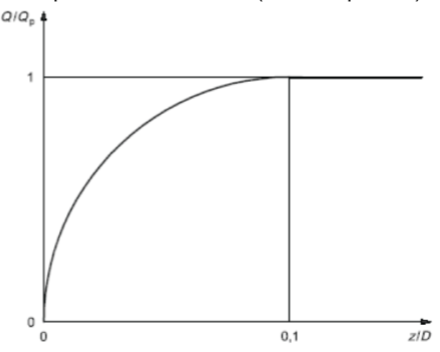
\includegraphics[scale=0.8]{pictures/part7/photo6.PNG}
\end{center} 

\subsection{Réduction de la longueur}

La diminution de longueur est donnée par l'équation de la rigidité :

$$ \Delta l = \frac{L F_{average}}{EA} $$

La force n'étant pas constante le long du pieu, la longueur de contraction élastique varie en fonction de la hauteur (plus comprimé en haut qu'en bas).

Risque de ramolissement de la couche (strain softening). Cela peu créer des rupture lorsque la couche à une capacité moindre à celle idéalisée. Au sommet, il u a plus de déplacement qu'au fond à cause de la différence de compression (réduction)

\subsection{IMPORTANT}

MAX END BEARING occuss after larger settlement than MAX SKIN FRICTION, friction strain softening may lead to reduced capacity !

\begin{center}
    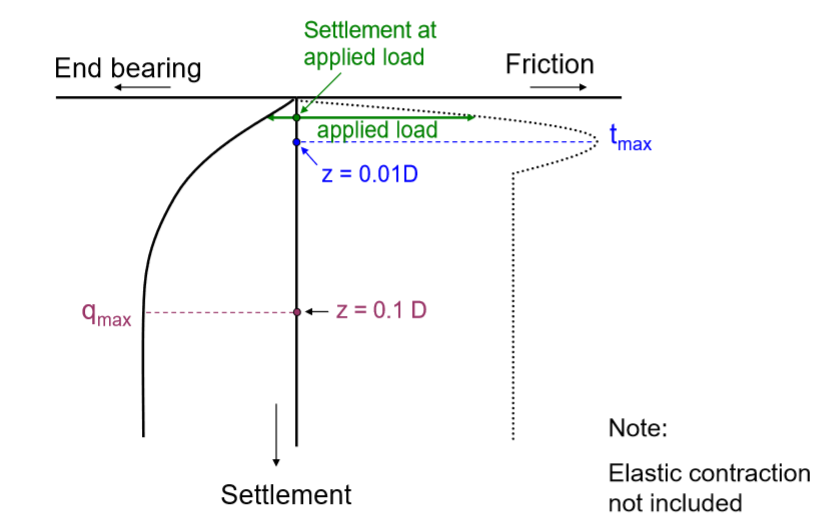
\includegraphics[scale=0.8]{pictures/part7/photo7.PNG}
\end{center} 

\section{Drivability}

C'est important car l'installation d'une barge est très cher. Il s'agit de la faisabilité d'atteindre une pénétration de la cible en poussant. Pour ça il faut sélectionner la combinaison pieu-marteau optimal en fonction du type de sol (permet de mieux choisir le type de pieu). Et analyser des donnée de fatigue de l'acier utilisé.

On se base sur la conservation d'énergie, la loi de Hooke (déformation élastique) et la loi de Newton.

Certain sols ne sont pas idéals pour ce genre de manoeuvre: Sols calcaires, limons, Mica sableux, Mudstone/siltStone, ...

\subsection{Hammer Types}


\begin{tabular}{c|c|c|c}
     & Water depths [m] & Energy range [kNm] & Hammer efficiency [\%] \\
     \hline
    Hydraulic Hammers & 50 - 300 & 1000 - 2100 & 90 - 100 \\
    Steam Hammers & 75 & 130 - 2200 & 60 - 75 \\
    Diesel Hammers & 75 & 20 - 70 & 60 - 75
\end{tabular}

\subsection{Hydraulic Hammer}

On porte le mouton avec un piston hydraulique, on peu ajuster la hauteur, la masse tombe sous son propre poids, on peut ajouter une force additionnelle avec un gaz comprimé (jusqu'à 2g).

\underline{Avantages :} Grande efficacité, fonctionne sous l'eau, installation rapide, bon rythme de frappe et un meilleur contrôle du processus (énergie et rythme). (pas besoin d'un coussin et marteau en acier).

\subsection{Steam Hammers}

Pareil que le hydraulic hammer mais on utilise de la vapeur plutôt qu'un fluide hydraulique. Il nécessite un coussin (en bois dur ou en Hamortex). Il n'est plus vraiment utilisé.

\subsection{Diesel Hammer (internal combustion)}

Fonctionne comme un moteur à deux temps. La mixture air-diesel explose et monte la masse jusqu'à son point le plus élevé. Le mouton descend en compressant la mixture, tombe sur l'enclume, allume la mixture et remonte. Il y a une énergie supplémentaire que celle de la chute qui est fournie (explosion). Un coussin est nécessaire et il y a une perte d'énergie avec le rebond.

\subsection{Soil Resistance to driving (SRD)}

Ce n'est pas égal à la capacité portante d'un pieu :

\begin{center}
\begin{tabular}{c|c}
$SRD = \sum f_e Ae + \sum f_iA_i + q_a A_W$
        &  $f_e$ : friction extérieur \\
        &  $A_e$ : air extérieur \\
        &  $f_i$ : friction intérieur \\
        &  $A_i$ : air intérieur \\
        &  $q_a$ : résistance à la base \\
        &  $A_W$ : section à la base
\end{tabular}
\end{center}

Ce n'est pas équivalent car SRD utilise de très grandes estimations contrairement à la capacité statique, Il y a un effet d'inertie du "plug", un remaniement des sols (argiles) et l'apparition de beaucoup de pression interstitielle à cause des grandes contraintes.

\subsection{Equation de la théorie des ondes}

On considère le pieu comme un grand nombre de segments représentable par des ressorts. On a donc une onde de compression qui se propage verticalement du à la pression généré par le marteau d'une vitesse $c = \sqrt{E/\rho}$ pour l'acier cela revient à environ 5100 m/s. (On peut calculer la ca par les équations de conservation d'énergie.

\begin{center}
\begin{tabular}{c|c}
$J = \xi c S_r$
        &  $J$ : amortissement  \\
        &  $\xi$ : facteur d'amortissement  \\
        &  $c$ : vitesse de l'onde  \\
        &  $S_r$ : résistance du sol
\end{tabular}
\end{center}

\newpage

\part{Pipeline Geotechnics}

\section{Pipe-Soil interaction modelling}

Lors du dimensionnement d'un modèle pipeline-sol, on aura besoin de connaître son diamètre extérieur total (D), son poids submergé (pendant l'installation (vide) $W_i$, inondé d'eau $W_f$, en service $W_{op}$), sa rugosité ($R_a$), sa rigidité à la torsion (EI) et la tension effective ressentie à l'installation au moment ou le pipe touche le sol ($T_0$).

Il faut ensuite choisir la route à prendre. On essaye de prendre les zones les plus plates possibles. Si la rugosité pose problème par endroit, on enlève ou rajoute des matériaux avant l'installation du pipe.

On rencontre différents défis de conception : 
\begin{center}
    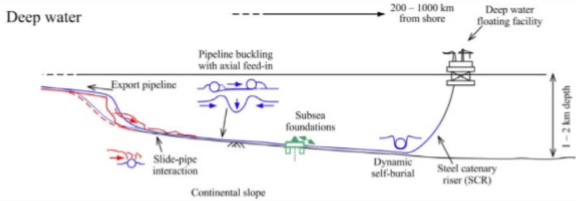
\includegraphics[scale=1]{pictures/part8/photo1.PNG}
\end{center} 
\begin{center}
    \includegraphics[scale=1]{pictures/part8/photo2.PNG}
\end{center} 

On rencontre des problèmes différents de ceux rencontré avec des fondations "basiques". A cause de la géométrie du pipe et des conditions océanique, le tuyau a tendance à s'auto enfoncer dans le sol ou au moins à dérangé les couches de fond marin. Pour le garder au maximum fixe, il faut que sont diamètre D soit beaucoup plus important que son enfoncement (u) "cyclique" dans le sol du au charge hydrodynamique. Finalement, la capacité géotechnique supérieure et inférieure peut avoir une incidence négative sur la réponse structurale.

\subsection{Objectifs}

Le but premier est de \textbf{réduire le risque} en minimisant les incertitudes géotechnique. On utilise des méthodes de sondage avec du matériel approprié, ...
Ensuite en essaye d'\textbf{optimiser la conception} en améliorant les techniques d'analyses des données recueillies (approche probalistique, software,...).
Finalement on cherche à \textbf{diminuer le prix} en améliorant les matériaux, diminuant les contraintes, diminuant les coûts de production et de mise en place.

\subsection{Ce qu'on essaye de quantifier}

On s'intéresse principalement aux efforts latéral, verticale et axial. L'interaction tuyau-sol comporte de grandes incertitude et constitue l'aspect le plus vital de la conception global de flambage ou d'expansion. La recherche dans ce domaine permettrait un grand gain de temps et d'argent (par exemple en réduisant les exigence des critères d'acceptation des soudures inter pipe). Ce forces interagissent directement avec les différents problèmes lié aux pipe : flambement latéral, l'arrachement de la courbe d'ancrage,...

\subsection{interaction}

Le dimensionnement du pipe à une influence sur les interactions sol-pipe et inversement. Ils faut donc allier pipeline geotechnics et pipeline engineering. 

La pénétration du tuyau dans le sol dépendra des propriété du sol (angle de friction, force de cisaillement,...) de ses conditions initiale (remblais ?) et de son passif (chargement passé ?).

La résistance axial et latéral du sol dépendra également des propriété du sol mais aussi du type de charge, de la durée de celle-ci, de la rugosité du pipe,...

\section{Installation du Pipe}

\begin{center}
    \includegraphics[scale=1]{pictures/part8/photo3.PNG}
\end{center} 

\begin{itemize}
    \item Il y a un renforcement de la capacité portante lors de la pose de la canalisation.
    \item La force change avec la pénétration cyclique du sol.
    \begin{center}
    \includegraphics[scale=1]{pictures/part8/photo4.PNG}
\end{center} 
\end{itemize}

\section{Dimensionnement}

\subsection{Modèle de pénétration vertical}

$$ \frac{V_{ult}}{S_{u,invert}D} = N_c + f_b \frac{A'\gamma'}{S_{u,invert}D} $$ 

\begin{center}
    honnêtement j'aurai essayé mais là ! 
    Voir slide 27 à 29 de la lecture8 
\end{center}

\subsection{Effort de cisaillement à l'interface}

\subsubsection{Residual Stress Ratio - Velocity}

\begin{center}
    \includegraphics[scale=0.8]{pictures/part8/photo5.PNG}
\end{center} 

\subsubsection{influence de la surconsolidation}

\begin{center}
    \includegraphics[scale=0.8]{pictures/part8/photo6.PNG}
\end{center} 

On observe une augmentation du frottement axial. Cela se produit lorsqu'on vide les pipes dans des conditions d'utilisations.

\subsubsection{influence of stress effects}

\begin{center}
    \includegraphics[scale=0.8]{pictures/part8/photo7.PNG}
\end{center} 

\subsubsection{Influence du temps (drainé ou non)}

\begin{center}
    \includegraphics[scale=0.8]{pictures/part8/photo8.PNG}
\end{center} 

Le temps de cisaillement affecte le niveau de drainage.

\subsection{influence de la consolidation cyclique}

\begin{center}
    \includegraphics[scale=0.8]{pictures/part8/photo9.PNG}
\end{center} 

\section{Réponse latérale des pipes lourds}

\begin{center}
    \includegraphics[scale=0.8]{pictures/part8/photo10.PNG}
\end{center} 

Les tuyaux les plus lourd peuvent se déplacer verticalement dans le sol après que la résistance de "breakout" soit mobilisée. Ce mouvement vers le bas couplé avec l'apparition de remblais sur le pipe le pousse à continuer sa descente. Ce genre de calcul devenant compliqué on utilise des logiciel pour les analyser.

\section{Some advices}

Différentes recommandations pour optimiser la mise en place de pipelines (selon fugro) :

Il est important d'engager des ingénieurs géotechniciens tôt dans le projet pour avoir dès le début des données géotechniques précise et utilisable. 

Utiliser dès le début des test en laboratoire et sur le site, tester les efforts de cisaillement à l'interface, surtout dans les zones ou l'on a peu d'info sur les fonds.

Encourager des échanges réguliers entre ingénieur géotechniciens et ingénieur de pipeline. Leur interaction est importantes pour palier à toutes éventualités.

Surveiller et analyser les résultats une fois le pipe mis en place pour s'en inspirer à l'avenir.

\section{Pipeline design exemple}

On peu effectuer de nombreuses analyse numérique. On peu par exemple optimiser la résistance au flambement latéral, flambement vertical (déplacement de cailloux). Optimiser la route ou les supports. Analyser les impacts de débris, la remonté des pipelines, ...

Il est maintenant possible dans les logiciel de modifier l'allure du fond marin, de modéliser les différentes couches du pipeline précisément, de considérer une excavation et un remblais. On peut ainsi prédire la forme que prendra le pipe à cause du flambement et précisément ou il flambera. Connaître les contraintes qu'il sentira au droit de sa section à différents endroits,... Bref on a pleins d'infos.

\end{document}
